\documentclass[12pt]{report}
\usepackage[utf8x]{inputenc}
\usepackage[russian]{babel}
\usepackage{amsmath}
\usepackage{graphicx}
\usepackage{enumitem}
\usepackage{titlesec}
\usepackage{tocloft}

\titleformat{\chapter}[display]
    {\filcenter}
    {\MakeUppercase{\chaptertitlename} \thechapter}
    {8pt}
    {\bfseries}{}

\titleformat{\section}
    {\normalsize\bfseries}
    {\thesection}
    {1em}{}

\titleformat{\subsection}
    {\normalsize\bfseries}
    {\thesubsection}
    {1em}{}


\makeatletter
    \AddEnumerateCounter{\asbuk}{\@asbuk}{м)}
\makeatother
\setlist{nolistsep}
\renewcommand{\labelitemi}{-}
\renewcommand{\labelenumi}{\asbuk{enumi})}
\renewcommand{\labelenumii}{\arabic{enumii})}

% Настройка вертикальных и горизонтальных отступов
\titlespacing*{\chapter}{0pt}{-30pt}{8pt}
\titlespacing*{\section}{\parindent}{*4}{*4}
\titlespacing*{\subsection}{\parindent}{*4}{*4}

\graphicspath{{graphic/chapter1/} {graphic/chapter2/} {graphic/chapter3/}}

\renewcommand{\labelenumii}{\arabic{enumi}.\arabic{enumii}}

\textwidth=15cm
\textheight=22cm
\oddsidemargin= 0.5cm
\topmargin = -0.5cm


%Настройка оглавления
\renewcommand{\cfttoctitlefont}{\hspace{0.38\textwidth} \bfseries\MakeUppercase}
\renewcommand{\cftbeforetoctitleskip}{-1em}
\renewcommand{\cftaftertoctitle}{\mbox{}\hfill \\ \mbox{}\hfill{\footnotesize Стр.}\vspace{-2.5em}}
\renewcommand{\cftchapfont}{\normalsize\bfseries \MakeUppercase{\chaptername} }
\renewcommand{\cftsecfont}{\hspace{31pt}}
\renewcommand{\cftsubsecfont}{\hspace{11pt}}
\renewcommand{\cftbeforechapskip}{1em}
\renewcommand{\cftparskip}{-1mm}
\renewcommand{\cftdotsep}{1}
\setcounter{tocdepth}{2} % задать глубину оглавления — до sub9section включительно


\begin{document}
Титульный Лист.
\newpage
\tableofcontents
\newpage

\chapter{Описание методов моделирования систем}
\section{Введение}

    В современном мире средства вычислительной техники широко используются во многих отраслях деятельности человека. Основной их задачей является обработка и хранение информации поступающей из вне. Такие системы должны обеспечивать доступ к данным и гарантировать их актуальность. Для решения проблемы быстрого получения информации конечным пользователям, отдельные компьютеры объединяются в локальные сети. Подобное объединение можно проследить вплоть до глобальной сети интернет. Однако, решив проблему, связанную с доступностью информации, соединение компьютеров обострило проблемы связанные с безопасностью данных. В случае с локальной машиной не имеющей активного сетевого соединения проблема безопасности решается ограничение физического доступа к терминалу, однако объединив рабочие станции, зона, которую необходимо контролировать, резко возрастает. Кроме того, с внедрением беспроводных технологий, это зона не имеет четких границ, а существующее подключение сети к интернет открывает потенциальную возможность для атаки человеку из любой точки мира. В зависимости от сложности архитектуры, от используемого оборудования и уровня подготовленности сотрудников, имеющих подключение к локальной сети, обнаружение и ликвидация уязвимостей резко возрастает. Принимая во внимание вышеперечисленные факторы, инженеру, ответственному за построение локальной сети, необходимо иметь возможность оценки того или иного архитектурного или программного решения с точки зрения актуальности его применения для конкретной ситуации. Для подобного рода оценок существуют различные методы и средства моделирования.

    Применение методов моделирования на этапе проектирования сети позволяет предугадать возможные проблемы при реализации выбранного решения, а также принять меры по обеспечению безопасного функционирования системы. К таким мерам относятся аппаратные средства, ограничивающие доступ к защищаемым ресурсам, протоколы криптографической защиты, программное обеспечение с возможностью мониторинга состояния сети. Различные источники придерживаются разных определений процесса моделирования, так как крайне сложно подобрать такое определение, которое в полной мере охватило деятельность по моделированию. Определение модели по А. А. Ляпунову: Моделирование – это опосредованное практическое или теоретическое исследование объекта, при котором непосредственно изучается не сам интересующий нас объект, а некоторая вспомогательная искусственная или естественная система (модель):

    \begin{itemize}
        \item находящаяся в некотором объективном соответствии с познаваемым объектом;
        \item способная замещать его в определенных отношениях;
        \item дающая при её исследовании, в конечном счете, информацию о самом моделируемом объекте;
    \end{itemize}

    "Модель (лат. modulus – мера) – это объект заместитель объекта-оригинала, обеспечивающий изучение некоторых свойств оригинала. Замещение одного объекта другим с целью получения информации о важнейших свойствах объекта-оригинала с помощью объекта-модели называется моделированием.Под математическим моделированием будем понимать процесс установления соответствия данному реальному объекту некоторого математического объекта, называемого математической моделью, иисследование этой модели, позволяющее получать характеристики рассматриваемого реального объекта. Вид математической модели зависит как от природы реального объекта, так и задач исследования объекта и требуемой достоверности и точности решения этой задачи."[1] Основная сложность математического моделирования заключается в том, что исследуемые процессы необходимо формализовать математическими функциями, что не всегда возможно. Некоторые процессы, например, действия пользователя в системе, сложно свести к математическим функциям.

    Имитационное моделирование – это метод, позволяющий строить модели, описывающие процессы так, как они проходили бы в действительности. Отличительными чертами данного метода является то, что у исследователя есть возможность изменять параметры системы, изучать процесс с одними входными данными или некоторым набором, исследовать развитие процесса во времени. Имитационное моделирование применяется тогда, когда неэффективно с точки зрения затраченных ресурсов и полученных результатов экспериментировать на реальном объекте. Невозможно построить математическую модель в связи с присутствующими в системе нелинейностях, стохастическими переменными или если необходимо исследовать систему во времени. Существующие программные решения позволяют строить модели компьютерных сетей, и исследовать с помощью этой модели различные процессы, происходящие в системе. Однако большинство таких решений созданы для использования системными администраторами, и поэтому позволяют исследовать характеристики системы безотносительно к безопасности. Данные, полученные при использовании такой системы, могут быть абсолютно бесполезными для инженера по безопасности. Существующие решения, отражающие работу сети с точки зрения безопасности являются коммерческими, что затрудняет их использование в образовательных целях или являются свободно распространяемыми, но в этом случае, обычно, обладают малым числом возможностей и неудобным для использования графическим интерфейсом. Таким образом целью данной работы является создание стенда для моделирования работы вычислительной сети с точки зрения информационной безопасности. Данный стенд должен предоставлять возможность построения сетей различных архитектур и топологий, выявлять "узкие"места в локальной сети замедляющие ее работу или представляющие собой уязвимость, а так же изучить состояние и поведение системы при различного рода атаках. В качестве объекта исследования будем рассматривать процесс моделирования взаимодействия различных устройств, объединенных в вычислительную сеть. В рамках данной работы будет построена система, позволяющая моделировать алгоритмы работы устройств на различных уровнях эталонной модели взаимодействия открытых систем(OSI). Протоколы транспортного сетевого и канального уровней возможно моделировать без привлечения математических моделей и аппарата математической статистики. В то время как более высокие уровни взаимодействия связаны с действиями пользователя в системе и не могут быть точно воспроизведены. В связи с этим при моделировании генерации трафика в сети, то есть обычного режима работы, будут использованы математические модели, построенные при исследовании данного явления. При моделировании работы протоколов нижнего уровня и физической передачи данных возникаю проблемы иного характера. Они связаны в первую очередь с наличием ошибки в канале связи. Учитывая то, что в реальных условиях эта ошибка носит, преимущественно, случайный характер, моделирование подобных инцидентов будет проводится с использованием методов математической статистки.

    Для построения модели вычислительной сети будет применен метод имитационного моделирования. Благодаря этому методу система будет иметь необходимую гибкость при настройке параметров. Наиболее удобным видом моделирования для данной задачи является метод агентного моделирования, так как он позволяет описывать поведение каждого компонента системы в отдельности, а так же порядок их взаимодействия. Описанные преимущества позволяют произвести декомпозицию задачи и построить систему необходимого уровня сложности.

    Для построения целевой системы необходимо разработать архитектуру будущего приложения. Она должна включать в себя возможности по построению моделей вычислительных сетей различной конфигурации, предусматривать механизмы настройки большинства компонентов системы, обладать гибкостью для возможного расширения используемого оборудования и протоколов. Следующим этапом разработки является алгоритмизация математических моделей, описывающих генерацию трафика пользователем в вычислительной сети. Результатом данного этапа будет система, в достаточной степени точно отражающая реальные процессы, протекающие в вычислительной сети. Третьим этапом разработки станет подсистема сбора статистической информации по различным устройствам. Данная подсистема занимается сбором данных со всех устройств, входящих в состав моделируемой сети и позволяет проследить динамику изменения состояний различных узлов. Заключительным этапом является создание подсистемы, моделирующей различные виды атак на локальную сеть. В рамках данной подсистемы описываются устройства и программы(алгоритмы), используемые при атаках на вычислительные сети, определяются механизмы подключение к локальной сети, моделируются действия злоумышленника. По последнему пункту будет рассмотрено такое понятие, как мотивация злоумышленника, которая влияет на его заинтересованность в компрометации системы.

    Для решения поставленных задач будет использоваться язык программирования JAVA с использованием различных расширений.




\section{Классификация видов моделирования.}

\subsection{Классификационные признаки.}

 В качестве одного из первых признаков классификации видов моделирования можно выбрать степень полноты модели и разделить модели в соответствии с этим на полные, неполные и приближенные. В основе полного моделирования лежит полное подобие, которо проявляется как во времени, так и в пространстве. Для неполного моделирования характерно неполное подобие модели изучаемому объекту. В основе приближенного моделирования лежит приближенное подобие, при котором некоторые стороны функционирования реального объекта не моделируются совсем.

    В зависимости от характера изучаемых процессов в системе S все виды моделирования могут быть разделены на детерминированные и стохастические, статические и динамические, дискретные, непрерывные и дискретно-непрерывные. Детерминированное моделирование отображает детерминированные процессы, т.е. процессы, в которых предполагается отсутствие всяких случайных воздействий; стохастическое моделирования отображает вероятностные процессы и события. В этом случае анализируется ряд реализаций случайного процесса и оцениваются средние характеристики, т.е. набор однородных реализаций. Статическое моделирования служит для описания поведения объекта в какой-либо момент времени, ф динамическое моделирование отражает поведение объекта во времени. Дискретное моделирование служит для описания процессов, которые предполагаются дискретными, соответственно непрерывное моделирование используется для случаев, когда хотят выделить наличие как дискретных, так и непрерывных процессов.[1]


\subsection{Математическое моделирование.}

 Для исследования характеристик процесса функционирования любой системы S математическими методами, включая и машинные, должна быть проведена формализация этого процесса, т.е. построена математическая модель.

    Под математическим моделированием понимают процесс установления соответствия данному реальному объекту некоторого математического объекта, называемого математической моделью, и исследование этой модели, позволяющее получать характеристики рассматриваемого реального объекта. Вид математического модели зависит как от природы реального объекта, так и задач исследования объекта и требуемой достоверности и точности решения этой задачи. Любая математическая модель, как и всякая другая описывает реальный объект лишь с некоторой степенью прближения к действительности. Математическое моделирование для исследвания характеристик процесса функционирования систем можно разделить на аналитическое, имитационное и комбинированное.

    Для аналитического моделирования характерно то, что процессы функционирования элементов системы записываются в виде некоторых функциональных соотношений (алгебраических, интегродифференциальных, конечно-разностных и.т.п.) или логических условий. Аналитическая модель может быть исследована следующими методами:
\begin{enumerate}
  \item аналитическим, когда стремятся получить в общем виде явные зависимости для искомых характеристик;
  \item численным, когда, не умея решать уравнений в общем виде, стремятся получить числовые результаты при конкретных начальных данных;
  \item качественным, когда, не имея решения в явном виде, можно найти некоторые свойства решения.
\end{enumerate}

    Наиболее полное исследование процесса функционирования системы можно провести, если известны явные зависимости, связывающие искомые характеристики с начальными условиями, параметрами и переменными системы S. Однако такие зависимости удается получить только для сравнительно простых систем. При усложнении систем исследование их аналитическим методом наталкивается на значительные трудности, которые часто бывают непреодолимыми. Поэтому, желая использовать аналитический метод, в этом случае идут на существенное упрощение первоначальной модели, чтобы иметь возможность изучить хотя бы общие свойства системы. Такое исследование на упрощенной модели аналитическим методом помогает получить ориентировочные результаты для определения более точных оценок другими методами. Численный метод позволяет исследовать по сравнению с аналитическим методом более широкий класс систем, но при этом полученные решения носят частный характер. Численный метод особенно эффективен при использовании ЭВМ.

    В отдельных случаях исследования системы могут удовлетворять и те выводы, которые можно сделать про использовании качественного метода анализа математической модели. Такие качественные методы широко используются, например, в теории автоматического управления для оценки эффективности различных вариантов систем управления.

    В настоящее время распространены методы машинной реализации исследования характеристик процесс функционирования больших систем. Для реализации математической модели на ЭВМ необходимо построить соответствующий моделирующий алгоритм.

    При имитационном моделировании реализующий модель алгоритм воспроизводит процесс функционирования системы S во времени, причем имитируются элементарные явления, составляющие процесс, с сохранением их логической структуры и последовательности протекания во времени , что позволяет по исходным данным получить сведения о состояниях процесса в определенные моменты времени, дающие возможность оценить характеристики системы S.

    Основным преимуществом имитационного моделирования по сравнению с аналитическим является возможность решения более сложных задач. Имитационные модели позволяют достаточно просто учитывать такие факторы, как наличие дискретных и непрерывных элементов, нелинейные характеристики элементов системы, многочисленные случайные воздействия и др., котоые часто создают трудности при аналитических исследованиях. В настоящее время имитационное моделирование -- наиболее эффективный метод исследования больших систем, а часто и единственный практически доступный метод получения информации о поведении системы, особенно на этапе ее проектирования.
    Когда результаты, полученные про воспроизведении на имитационной модели процесса функционирования системы S, являются реализациями случайных величин и функций, тогда для нахождения характеристик процесса требуется его многократное воспроизведение с последующей статистической обработкой информации и целесообразно в качестве метода машинной реализации имитационной модели использовать метод статистического моделирования. Первоначально был разработан метод статистических испытаний, представляющий собой численный метод, который применялся для моделирования случайных величин и функций, вероятностные характеристики которых совпадали с решениями аналитических задач (такая процедура получила название метода Монте-Карло). Затем этот прием стали применять и для машинной имитации с целью исследования характеристик процессов функционирования систем, подверженных случайным воздействиям, т.е. появился метод статистического моделирования. Таким образом, методом статистического моделирования называют метод машинной реализации имитационной модели, а методом статистических испытаний -- численный метод решения аналитической задачи.

    Метод имитационного моделирования позволяет решать задачи анализа больших систем, включая задачи оценки: вариантов структуры систем, эффективности различных алгоритмов управления системой, влияния изменения различных параметров системы. Имитационное моделирование может быть положено также в основу структурного. алгоритмического и параметрического синтеза больших систем, когда требуется создать систему, с заданными характеристиками при определенных ограничениях, которая является оптимальной по некоторым критериям оценки эффективности.

    При решении задач машинного синтеза систем на основе их имитационных моделей помимо разработки моделирующих алгоритмов для анализа фиксированной системы необходимо так же разработать алгоритмы поиска оптимального варианта системы. Далее в методологии машинного моделирования будем различать два основных раздела: статику и динамику, -- основным содержанием которых являются соответственно вопросы анализа и синтеза систем, заданных моделирующими алгоритмами.

    Комбинированное (аналитико-имитационное) моделирование при анализе и синтезе систем позволяет объединить достоинства аналитического и имитационного моделирования. При построении комбинированных моделей проводится предварительная декомпозиция процесса функционирования объекта на составляющие подпроцессы и для тех из них, где это возможно, используются аналитические модели, а для остальных подпроцессов строятся имитационные модели. Такой комбинированный подход позволяет охватить качественно новые классы систем, которые не могут быть исследованы с использованием только аналитического и имитационного моделирования в отдельности.[1]


\subsubsection{Формальная модель объекта.}

Модель объекта моделирования, т. е. системы S, можно представить в виде множества величин, описывающих процесс функционирования реальной системы и образующих в общем случае следующие подмножества:

\begin{enumerate}
  \item совокупность входных воздействий на систему
      \begin{center}
        $x_{i} \in X, i = \sup{1, n_{X}}$; х,еХ, i=l , пх;
      \end{center}

  \item совокупность воздействий внешней среды
     \begin{center}
       $\upsilon_{l} \in V l = \sup{1, n_{V}}$;
     \end{center}

  \item совокупность внутренних (собственных) параметров системы
     \begin{center}
       $h_{k} \in H, k = \sup{1, n_{H}}$;
     \end{center}

  \item совокупность выходных характеристик системы
    \begin{center}
      $y_{j} \in Y, j = \sup{1, n_{Y}}$
    \end{center}

\end{enumerate}

  При этом в перечисленных подмножествах можно выделить управляемые и неуправляемые переменные. В общем случае $x_{i}$, $\upsilon_{l}$, $h_{k}$, $y_{j}$ являются элементами непересекающихся подмножеств и содержат как детерминированные, так и стохастические составляющие. При моделировании системы S входные воздействия, воздействия внешней среды Е и внутренние параметры системы являются независимыми (экзогенными) переменными, которые в векторной форме имеют соответственно вид $\vec{x}(t) = (x_{1}(t), x_{2}(t), ..., x_{nX}(t))$; $\vec{v}(t) = (v_{1}(t), v_{2}(t), ... , v_{nV}(t))$; $\vec{h}(t) = (h_{1}(t), h_{2}(t), ... , h_{nH}(t))$, а выходные характеристики системы являются зависимыми (эндогенными) переменными и в векторной форме имеют вид $\vec{y}(t) = (y_{1}(t), y_{2}(t), ... , y_{nY}(t))$.

  Процесс функционирования системы S описывается во времени оператором Fs, который в общем случае преобразует экзогенные переменные в эндогенные в соответствии с соотношениями вида

  \begin{center}
    $\vec{y}(t) = F_{s}(\vec{x}, \vec{\upsilon}, \vec{h}, t)$
  \end{center}

  Совокупность зависимостей выходных характеристик системы от времени $y_{j}(t)$ для всех видов $j = \sup{1, n_{y}}$ называется выходной траекторией $\vec{y}(t)$. Зависимость (2.1) называется законом функционирования системы S и обозначается $F_{s}$. В общем случае закон функционирования системы $F_{s}$ может быт задан в виде функции, функционала, логических условий, в алгоритмической и табличной формах или в виде словесного правила соответствия. Весьма важным для описания и исследования системы S является понятие алгоритма функционирования $A_{s}$, под которым понимается метод получения выходных характеристик с учетом входных воздействий $\vec{x}(t)$, воздействий внешней среды $\vec{\upsilon}(t)$ и собственных параметров системы $\vec{h}(t)$. Очевидно, что один и тот же закон функционирования $F_{s}$ системы S может быть реализован различными способами, т. е. с помощью множества различных алгоритмов функционирования $A_{s}$. Соотношения (2.1) являются математическим описанием поведения объекта (системы) моделирования во времени t, т. е. отражают его динамические свойства. Поэтому математические модели такого вида принято называть динамическими моделями (системами).

  Для статических моделей математическая модель (2.1) представляет собой отображение между двумя подмножествами свойств моделируемого объекта Y и \{X, V, Н\}, что в векторной форме может быть записано как

  \begin{center}
      $\vec{y} = f(\vec{x}, \vec{\upsilon}, \vec{h})$.(2.2)
  \end{center}

  Соотношения (2.1) и (2.2) могут быть заданы различными способами: аналитически (с помощью формул), графически, таблично и т. д. Такие соотношения в ряде случаев могут быть получены через свойства системы S в конкретные моменты времени, называемые состояниями. Состояние системы S характеризуется векторами

  \begin{center}
    $\vec{z}' = (z_{1}', z_{2}', ... , z_{k}')$ и $\vec{z}'' = (z_{1}'', z_{2}'', ... , z_{k}'')$,
  \end{center}


  где $z_{1}'= z_{1}(t'), z_{2}' = z_{2}(t'), ... , z_{k}' = z_{k}(t')$ в момент $t' \in (t_{0}, T)$, $z_{1}'' = z_{1}(t''), z_{2}'' = z_{2}(t''), ... , z_{k}'' = z_{k}(t'')$  в момент $t'' \in (t_{0}, T)$ и т. д., $k = \sup{1, n_{z}}$. Если рассматривать процесс функционирования системы S как последовательную смену состояний $z_{1}(t), z_{2}(t), ... , z_{k}(t)$, то они могут быть интерпретированы как координаты точки в k-мерном фазовом пространстве, причем каждой реализации процесса будет соответствовать некоторая фазовая траектория. Совокупность всех возможных значений состояний $\{\vec{z}\}$ называется пространством состояний объекта моделирования Z, причем $z_{k} \in Z$.

  Состояния системы S в момент времени $t_{0} < t* <= T $ полностью определяются начальными условиями $\vec{z}^{0} = (z^{0}_{1}, z^{0}_{2}, ... , z^{0}_{k})$ [где $z^{0}_{1} = z_{1}(t_{0}), z^{0}_{2} = z_{2}(t_{0}), ... , z^{0}_{k} = z_{k}(t_{0})$], входными воздействиями $\vec{x}(t)$, внутренними параметрами $\vec{h}(t)$ и воздействиями внешней среды $\vec{\upsilon}(t)$, которые имели место за промежуток времени t* -- $t_{0}$, с помощью двух векторных уравнений

  \begin{center}
     $z(t) = \Phi(\vec{z}_{0}, \vec{x}, \vec{\upsilon}, \vec{h}, t)$ (2.3)

     $\vec{y}(t) = F(\vec{z}, t)$ (2.4)
  \end{center}


  Первое уравнение по начальному состоянию $\vec{z}^{0}$ и экзогенным переменным $\vec{x}, \vec{\upsilon}, \vec{h}$ определяет вектор-функцию $\vec{z}(t)$, а второе по полученному значению состояний $\vec{z}(t)$ — эндогенные переменные на выходе системы $\vec{y}(t)$. Таким образом, цепочка уравнений объекта «вход — состояния — выход» позволяет определить характеристики системы

  \begin{center}
    $\vec{y}(t) = F[\Phi(\vec{z}^{0}, \vec{x}, \vec{\upsilon}, \vec{h}, t)]$. (2.5)
  \end{center}

  В общем случае время в модели системы S может рассматриваться на интервале моделирования (0, Т) как непрерывное, так и дискретное, т. е. квантованное на отрезки длиной $\delta t$ временных единиц каждый, когда $T = m\delta t$, где $m = \sup{1,m_{T}}$ — число интервалов дискретизации.

  Таким образом, под математической моделью объекта (реальной системы) понимают конечное подмножество переменных \{ $\vec{x}(t), \vec{\upsilon}(t), \vec{h}(t) $\}вместе с математическими связями между ними и характеристиками $\vec{y}$.

  Если математическое описание объекта моделирования не содержит элементов случайности или они не учитываются, т. е. если можно считать, что в этом случае стохастические воздействия внешней среды $\vec{\upsilon}(t)$ и стохастические внутренние параметры $\vec{h}(t)$ отсутствуют, то модель называется детерминированной в том смысле, что характеристики однозначно определяются детерминированными входными воздействиями

  \begin{center}
    $\vec{y}(t) = f(\vec{x}, t)$. (2.6)
  \end{center}

  Очевидно, что детерминированная модель является частным случаем стохастической модели.

\subsubsection{Математическая схема.}

  Математическую схему можно определить как звено при переходе от содержательного к формальному описанию процесса функционирования системы с учетом воздействия внешней среды, т. е имеет место цепочка «описательная модель — математическая схема — математическая [аналитическая или (и) имитационная] модель».

  Каждая конкретная система S характеризуется набором свойств под которыми понимаются величины, отражающие поведение моделируемого объекта (реальной системы) и учитывающие условия ее функционирования во взаимодействии с внешней средой (системой) Е. При построении математической модели системы необходимо решить вопрос об ее полноте. Полнота модели регулируется в основном выбором границы «система S — среда Е». Также должна быть решена задача упрощения модели, которая помогает выделить основные свойства системы, отбросив второстепенные. Причем отнесение свойств системы к основным или второстепенным существенно зависит от цели моделирования системы (например, анализ вероятностно-временных характеристик процесса функционирования системы, синтез структуры системы и т. д.).

  Приведенные математические соотношения представляют собой математические схемы общего вида и позволяют описать широкий класс систем. Однако в практике моделирования объектов в области системотехники и системного анализа на первоначальных этапах исследования системы рациональнее использовать типовые математические схемы: дифференциальные уравнения, конечные и вероятностные автоматы, системы массового обслуживания, сети Петри и т. д.

  Не обладая такой степенью общности, как рассмотренные модели, типовые математические схемы имеют преимущества простоты и наглядности, но при существенном сужении возможностей применения. В качестве детерминированных моделей, когда при исследовании случайные факторы не учитываются, для представления систем, функционирующих в непрерывном времени, используются дифференциальные, интегральные, интегродифференциальные и другие уравнения, а для представления систем, функционирующих в дискретном времени,— конечные автоматы и конечно-разностные схемы. В качестве стохастических моделей (при учете случайных факторов) для представления систем с дискретным временем используются вероятностные автоматы, а для представления системы с непрерывным временем — системы массового обслуживания и т. д.

  Перечисленные типовые математические схемы, естественно, не могут претендовать на возможность описания на их базе всех процессов, происходящих в больших информационно-управляющих системах. Для таких систем в ряде случаев более перспективным является применение агрегативных моделей. Агрегативные модели (системы) позволяют описать широкий круг объектов исследования с отображением системного характера этих объектов. Именно при агрегативном описании сложный объект (система) расчленяется на конечное число частей (подсистем), сохраняя при этом связи, обеспечивающие взаимодействие частей.

  Таким образом, при построении математических моделей процессов функционирования систем можно выделить следующие основные подходы: непрерывно-детерминированный (например, дифференциальные уравнения); дискретно-детерминированный (конечные автоматы); дискретно-стохастический (вероятностные автоматы); непрерывно-стохастический (системы массового обслуживания); обобщенный, или универсальный (агрегативные системы).[1]

 \subsubsection{D-схемы}

 Обычно в таких математических моделях в качестве независимой переменной, от которой зависят неизвестные искомые функции, служит время t. Тогда математическое соотношение для детерминированных систем в общем виде будет

 \begin{center}
    $\vec{y}'= \vec{f}(\vec{y}, t), \vec{y}(t_{0}) = \vec{y}_{0}$
 \end{center}

 где $\vec{y}' = \dfrac{d\vec{y}}{dt}$,$\vec{y} = (y_{1}, y_{2}, ... , y_{n})$ и $\vec{f} = (f_{1}, f_{2}, ... , f_{n})$ -- n-мерные векторы;$f(\vec{y}, \vec{t})$ -- вектор-функция, которая определена на некотором (n + 1)-мерном $(\vec{y}, t)$ множестве и является непрерывной. Так как математические схемы такого вида отражают динамику изучаемой системы, т. е. ее поведение во времени, то они называются D-схемами (англ. dynamic).

 В простейшем случае обыкновенное дифференциальное уравнение имеет вид

  \begin{center}
    $y' = f(y, t)$
  \end{center}
 Наиболее важно для системотехники приложение D-схем в качестве математического аппарата в теории автоматического управления.[1]

    Процессы, которые могут быть описаны D-схемами являются сложными для моделирования, так как зависят от поведения пользователя. Однако, подобное описание пользовательских процессов приближает характеристики модели к реальным характеристика исследуемых процессов. В проектируемой системе необходимо предусмотреть способ генерации трафика рабочими станциями в системе. Существует несколько методов описания этого процесса.

    Пуассоновское распределение долгое время использовалось в имитационных моделях, как основа для функции генерации трафика, однако, исследования показали, что данный подход дает завышенную оценку производительности системы при режимах высокой нагрузки.[3] Другим подходом является использование аналитического метода описания процесса (D-схемы)[2]. Данный метод позволяет определить интенсивность трафика в зависимости от времени. Отличительной чертой такого подхода является точность описания процесса, однако использование предложенной модели является нецелесообразным в силу характера проектируемой системы.

    Наиболее подходящим методом для моделирования процесса генерации трафика является метод имитационного моделирования. Последние исследования говорят о статистическом самоподобии трафика[4]. Для генерации такого рода трафика следует использовать фрактальные модели[3].

 \subsubsection{Дискретно-детерминированные модели. (F -- схемы)}

 Особенности дискретно-детерминированного подхода на этапе формализации процесса функционирования систем рассмотрим на примере использования в качестве математического аппарата теории автоматов. Теория автоматов — это раздел теоретической кибернетики, в котором изучаются математические модели — автоматы. На основе этой теории система представляется в виде автомата, перерабатывающего дискретную информацию и меняющего свои внутренние состояния лишь в допустимые моменты времени. Понятие «автомат» варьируется в зависимости от характера конкретно изучаемых систем, от принятого уровня абстракции й целесообразной степени общности.

 Автомат можно представить как некоторое устройство (черный ящик), на которое подаются входные сигналы и снимаются выходные и которое может иметь некоторые внутренние состояния. Конечным автоматом называется автомат, у которого множество внутренних состояний и входных сигналов (а следовательно, и множество выходных сигналов) являются конечными множествами. Абстрактно конечный автомат (англ. finite automata) можно представить как математическую схему (F-схему), характеризующуюся шестью элементами: конечным множеством X входных сигналов (входным алфавитом); конечным множеством Y выходных сигналов (выходным алфавитом); конечным множеством Z внутренних состояний (внутренним алфавитом или алфавитом состояний); начальным состоянием $z_{0}, z_{0} \in Z $; функцией переходов $\phi(z, x)$; функцией выходов $\psi(z, x)$. Автомат, задаваемый F-схемой: $F = <Z, X, Y, \phi, \psi, z_{0}>$, -- функционирует в дискретном автоматном времени, моментами которого являются такты, т. е. примыкающие друг к другу равные интервалы времени, каждому из которых соответствуют постоянные значения входного и выходного сигналов и внутренние состояния.

 Абстрактный конечный автомат имеет один входной и один выходной каналы. В каждый момент t=0, 1, 2, ... дискретного времени F-автомат находится в определенном состоянии z(t) из множества Z состояний автомата, причем в начальный момент времени t = 0 он всегда находится в начальном состоянии $z(0) = z_{0}$ . В момент t, будучи в состоянии z(j), автомат способен воспринять на входном канале сигнал $x(t) \in X$ и выдать на выходном канале сигнал $y{t} = \psi[z(t), x{t}]$, переходя в состояние $z(t+1) = \phi[z(t), x(t)], z(t) \in Z, y(t) \in Y$. Абстрактный конечный автомат реализует некоторое отображение множества слов входного алфавита X на множество слов выходного алфавита Y.[1]

    Системы обработки данных, передаваемых по локальной сети по большей части построены как конечные автоматы. Наглядно данные вид моделей можно заметить при исследовании транспортной подсистемы, входящей в состав стека протоколов TCP/IP[5]. Поэтому модели протоколов следует строить с использованием(F-схем).

\subsubsection{Сетевые модели. (N - схемы.)}

  В практике моделирования объектов часто приходится решать задачи, связанные с формализованным описанием и анализом причинно-следственных связей в сложных системах, где одновременно параллельно протекает несколько процессов. Самым распространенным в настоящее время формализмом, описывающим структуру и взаимодействие параллельных систем и процессов, являются сети Петри.

  Теория сетей Петри развивается в нескольких направлениях: разработка математических основ, структурная теория сетей, различные приложения (параллельное программирование, дискретные динамические системы и т. д.).

  Формально сеть Петри (N-схема) задается четверкой вида

  \begin{center}
    $N = <B, D, I, O>$
  \end{center}

  где В — конечное множество символов, называемых позициями, $B \ne \oslash$; D — конечное множество символов, называемых переходами, $D \ne \oslash$ , $B \cap D \ne \oslash$; I—входная функция (прямая функция инцидентности), $I \colon B \times D\to \{0, 1\}$; О — выходная функция (обратная функция инцидентности), $O \colon D \times B \to \{0, 1\} $. Таким образом, входная функция I отображает переход $d_{I}$ в множество входных позиций $ b_{i} \in I(d_{j})$, а выходная функция О отображает переход $d_{j}$ в множество выходных позиций $b_{i} \in D(d_{j})$. Для каждого перехода $d_{j} \in D$ можно определить множество входных позиций перехода $I(d_{j})$ и выходных позиций перехода $O(d_{j})$

  \begin{center}
    $I(d_{j}) = \{b_{i} \in B|I(b_{i}, d_{j}) = 1\}$
  \end{center}

  \begin{center}
    $i = \sup{1,n}, j = \sup{1, m}, n = |B|, m = |D|$
  \end{center}

  \begin{center}
    $O(d_{j}) = \{b_{i} \in B|I(d_{j}, b_{i}) = 1\}$
  \end{center}

  Аналогично, для каждого перехода $b_{i} \in B$ вводятся определения множества входных переходов позиции $I(b_{i})$ и множества выходных переходов позиции $O(b_{i})$:

  \begin{center}
    $I(b_{i}) = \{d_{j} \in D|I(d_{j}, b_{i}) = 1 \}$
    `
    $O(b_{i}) = \{d_{j} \in D|O(b_{i}, d_{j}) = 1 \}$
  \end{center}

  Графически N-схема изображается в виде двудольного ориентированного мультиграфа, представляющего собой совокупность позиций и переходов. Как видно из этого рисунка, граф N-схемы имеет два типа узлов: позиции и переходы, изображаемые 0 и 1 соответственно. Ориентировочные дуги соединяют позиции и переходы, причем каждая дуга направлена от элемента одного множества (позиции или перехода) к элементу другого множества (переходу или позиции). Граф N-схемы является мультиграфом, так как он допускает существование кратных дуг от одной вершины к другой.

    Сети Петри с успехом применяются при моделировании различных процессов связанных с безопасностью систем[8][9]. Данный вид математических схем представляет широкий набор возможностей для моделирования динамических систем, в том числе, систем передачи трафика. Недостатком такого подхода в рамках решаемой задачи является высокий уровень абстракции N-схем, что влечет за собой необходимость специальных знаний для их использования.

\subsection{Имитационное моделирование.}

    Имитационное моделирование есть процесс конструирования модели реальной системы и постановки эксперимента на этой модели с целью либо понять поведение, либо оценить( в рамках ограничений, накладываемых некоторым критерием или совокупностью критериев) различные стратегии, обеспечивающие функционирование данной системы. Таким образом процесс имитационного моделирования мы понимаем как процесс, включающий и конструирование модели и, и аналитическое применение модели для изучения некоторой проблемы. Под моделью реальной системы понимается представление группы объектов или идей в некоторой форме, отличной от их реального воплощения; отсюда термин "реальный" используется в смысле "существующий или способный принять одну из форм существования".

    Имитационное моделирование является экспериментальной и прикладной методологией, имеющей целью:

\begin{itemize}
    \item описать поведение системы.
    \item построить теории и гипотезы, которые могут объяснить наблюдаемой поведение;
    \item использовать эти теории для предсказания будущего поведения системы, т.е. тех воздействий, которые могут быть вызваны изменениями в системе или изменениями способов ее функционирования.
\end{itemize}

  Идея представления некоторого объекта или понятия при помощи модели носит столь общий характер, что дать полную классификацию всех функций модели затруднительно. Можно выделить по крайней мере пять ставших привычными случаев применения моделей в качестве:

\begin{itemize}
    \item средства осмысления действительности,
    \item средства общения,
    \item средства обучения и тренажа,
    \item инструмента прогнозирования,
    \item средства постановки экспериментов.
\end{itemize}

    Все имитационные модели представляют собой модели типа так называемого черного ящика. Это означает, что они обеспечивают выдачу выходного сигнала системы, если на ее взаимодействующие подсистемы воздействует входной сигнал. Поэтому для получения необходимой информации или результатов необходимо осуществлять "прогон" имитационных моделей, а не "решать" их. Имитационные модели не способны формировать свое собственное решение в том виде, в котором это имеет место в аналитических моделях, а могут лишь служить в качестве средства для анализа поведения систем в условиях, которые определяются экспериментатором. Следовательно имитационное моделирование -- не теория, а методология решения проблем.[10]
    Имитационное моделирование есть экспериментирование с моделью реальной системы. Необходимость решения задачи путем экспериментирования становится очевидной, когда возникает потребность получить о системе специфическую информацию, которую нельзя найти в известных источниках. Непосредственное экспериментирование с на реальной системе устраняет множество затруднений, если необходимо обеспечить соответствие между моделью и реальными условиями; однако недостатки такого экспериментирования иногда весьма значительны, поскольку:

\begin{enumerate}
    \item Оно может нарушить установленный порядок работы фирмы.
    \item Если составной частью системы являются люди, то на результаты экспериментов может повлиять так называемый хауторнский эффект, проявляющийся в том, что люди, чувствуя, что за ними наблюдают, могут изменить свое поведение.
    \item Может оказаться сложным поддержание одних и тех же рабочих условий при каждом повторении эксперимента, или в течении всего времени проведении серии экспериментов.
    \item Для получения одной и той же величины выборки(и, следовательно, статистической значимости результатов эксперимента) могут потребоваться чрезмерные затраты времени и средств.
    \item При экспериментировании с реальными системами может оказаться невозможным исследование множества альтернативных вариантов.
\end{enumerate}

    При этом необходимо рассмотреть целесообразность применения имитационного моделирования при наличии любого из следующих условий:

\begin{enumerate}
    \item Не существует законченной математической постановки данной задачи, либо еще не разработаны аналитические методы решения сформулированной математической модели.
    \item Аналитические методы имеются, но математические процедуры столь сложны, что имитационное моделирование дает более простой способ решения задачи.
    \item Аналитические решения существуют, но их реализация невозможна в следствие не достаточной математической подготовки имеющегося персонала.
    \item Кроме оценки определенных параметров, желательно осуществить на имитационной модели наблюдение за ходом процесса в течение определенного времени.
    \item Имитационное моделирование может оказаться единственной возможностью вследствие трудностей трудностей постановки экспериментов и наблюдения явлений в реальных условиях.
    \item Для долговременного действия систем или процессов может понадобиться сжатие временной шкалы.
\end{enumerate}

\subsubsection{Виды имитационного моделирования.}

    По способу описания процессов моделируемой системы можно выделить три вида имитационного моделирования:

\begin{itemize}
    \item Агентное моделирование -- используется для исследования децентрализованных систем, динамика функционирования которых определяется не глобальными правилами и законами (как в других парадигмах моделирования), а наоборот, когда эти глобальные правила являются результатом индивидуальной активности членов группы. Цель агентных моделей -- получить представление об этих глобальных правилах, общем поведении системы, исходя из предположений об индивидуальном, частом поведении ее ее отдельных активных объектов и взаимодействии этих объектов в системе. Агент -- некая сущность, обадающая активностью, автономным поведением, может принимать решения в соответствии с некоторым набором правил, взаимодействовать с окружением, а так же самостоятельно изменяться.
    \item Дискретно-событийное моделирование -- подход к моделированию, предлагающий абстрагироваться от непрерывной природы событий и рассматривать только основные события моделируемой системы, такие как "ожидание", "обработка заказа", "движение с грузом", "разгрузка" и другие. Дискретно-событийное моделирование наиболее развито и имеет огромную сферу приложений -- от логистики и систем массового обслуживания до транспортных и производственных систем. Этот вид моделирования наиболее подходит для моделирования производственных процессов.
    \item Системная-динамика - парадигма моделирования, где для исследуемой системы строятся графические диаграммы причинных связей и глобальных влияних одних параметров на другие во времени, а затем созданная на основе этих диаграмм модель имитируется на компьютере. По сути, такой вид моделирования позволяет более всех других парадигм понять суть происходящего выявления причинно-следственных связей между объектами и явлениями.
\end{itemize}

\subsection{Языки имитационного моделирования.}

    Для моделирования систем используются как универсальные и процедурно-ориентированные языки общего назначения(ЯОН), так и специализированные языки имитационного моделирования(ЯИМ). При этом ЯОН предоставляют программисту-разработчику модели $M_{M}$ больше возможностей в смысле гибкости разработки, отладки и использования модели. Но гибкость приобретается ценой больших усилий, затрачиваемых на программирование модели, так как организация выполнения операций, отсчет системного времени и контроль хода вычислений существенно усложняются.

    Имеющиеся ЯИМ можно разбить на три основные группы, соответствующие трем типам математических схем: непрерывные, дискретные и комбинированные. Языки каждой группы предназначены для соответствующего представления системы S при создании ее машинной модели $M_{M}$.

    В основе рассматриваемой классификации в некоторых ЯИМ лежит принцип формирования системного времени. Так как «системные часы» предназначены не только для продвижения системного времени в модели Мм, но также для синхронизации различных событий и операций в модели системы S, то при отнесении того или иного конкретного языка моделирования к определенному типу нельзя не считаться с типом механизма «системных часов».

    Непрерывное представление системы S сводится к составлению уравнений, с помощью которых устанавливается связь между эндогенными и экзогенными переменными модели. Примером такого непрерывного подхода является использование дифференциальных уравнений. Причем в дальнейшем дифференциальные уравнения могут быть применены для непосредственного получения характеристик системы, это, например, реализовано в языке MIMIC. А в том случае, когда экзогенные переменные модели принимают дискретные значения, уравнения являются разностными. Такой подход реализован, например, в языке DYNAMO.

    Представление системы S в виде типовой схемы, в которой участвуют как непрерывные, так и дискретные величины, называется комбинированным. Примером языка, реализующего комбинированный подход, является GASP, построенный на базе языка FORTRAN. Язык GASP включает в себя набор программ, с помощью которых моделируемая система S представляется в следующем виде. Состояние модели системы М (S) описывается набором переменных, некоторые из которых меняются во времени непрерывно. Законы изменения непрерывных компонент заложены в структуру, объединяющую дифференциальные уравнения и условия относительно переменных. Предполагается, что в системе могут наступать события двух типов: 1) события, зависящие от состояния $z_{j}$, 2) события, зависящие от времени $t_{i}$. События первого типа наступают в результате выполнения условий, относящихся к законам изменения непрерывных переменных. Для событий второго типа процесс моделирования состоит в продвижении системного времени от момента наступления события до следующего аналогичного момента. События приводят к изменениям состояния модели системы и законов изменения непрерывных компонент. При использовании языка GASP на пользователя возлагается работа по составлению на языке FORTRAN подпрограмм, в которых он описывает условия наступления событий, зависящих от процесса функционирования системы S, законы изменения непрерывных переменных, а также правила перехода из одного состояния в другое.

    В рамках дискретного подхода можно выделить несколько принципиально различных групп ЯИМ. Первая группа ЯИМ подразумевает наличие списка событий, отличающих моменты начала выполнения операций. Продвижение времени осуществляется по событиям, в моменты наступления которых производятся необходимые операции, вклю­
чая операции пополнения списка событий. Примером языка событий является язык SIMSCRIPT. Разработчики языка SIMSCRIPT исходили из того, что каждая модель $M_{M}$ состоит из элементов, с которыми происходят события, представляющие собой последовательность предложений, изменяющих состояния моделируемой системы в различные моменты времени.

    При использовании ЯИМ второй группы после пересчета системного времени, в отличие от схемы языка событий, просмотр действий с целью проверки выполнения условий начала или окончания какого-либо действия производится непрерывно. Просмотр действий определяет очередность появления событий. Языки данного типа имеют в своей основе поисковый алгоритм, и динамика системы S описывается в терминах действий. Примером языка действий (работ) является ЯИМ FORSIM, представляющий собой пакет прикладных программ, который позволяет оперировать только фиксированными массивами данных, описывающих объекты моделируемой системы. С его помощью нельзя имитировать системы переменного состава. При этом размеры массивов  устанавливаются либо во время компиляции программы, либо в самом начале ее работы. Язык FORSIM удобен для описания систем с большим числом разнообразных ресурсов, так как он позволяет записывать условия их доступности в компактной форме. Конкретный способ формализации модели на языке действий в достаточной степени произволен и остается на усмотрение программиста, что требует его достаточно высокой квалификации. Полное описание динамики модели $M_{M}$ можно получить с помощью разных наборов подпрограмм.

    Третья группа ЯИМ описывает системы, поведение которых определяется процессами. В данном случае под процессом понимается последовательность событий, связь между которыми устанавливается с помощью набора специальных отношений. Динамика заложена в независимо управляемых программах, которые в совокупности составляют программу процесса. Пример языка процессов — язык SIMULA, в котором осуществляется блочное представление моделируемой системы S c использованием понятия процесса для формализации элементов, на которые разбивается моделируемая система. Процесс задается набором признаков, характеризующих его структуру, и программой функционирования. Функционирование каждого процесса разбивается на этапы, протекающие в системном времени.

    Главная роль в языке SIMULA отводится понятию параллельного оперирования с процессами в системном времени, а также универсальной обработке списков с процессами в роли компонент. Специальные языковые средства предусмотрены для манипуляций с упорядоченными множествами процессов.

    В отдельную группу могут быть выделены ЯИМ типа GPSS, хотя принципиально их можно отнести к группе языков процессов. Язык GPSS представляет собой интерпретирующую языковую систему, применяющуюся для описания  пространственного движения объектов. Такие динамические объекты в языке GPSS называются транзактами и представляют собой элементы потока. В процессе имитации транзакты «создаются» и «уничтожаются». Функцию каждого из них можно представить как движение через модель $M_{M}$ с поочередным воздействием на ее блоки. Функциональный аппарат языка образуют блоки, описывающие логику модели, сообщая транзактам, куда двигаться и что делать дальше. Данные для ЭВМ подготавливаются в виде пакета управляющих и определяющих карт, который составляется по схеме модели, набранной из стандартных символов. Созданная GPSS-программа, работая в режиме интерпретации, генерирует и передает транзакты из блока в блок в соответствии с правилами, устанавливаемыми блоками. Каждый переход транзакта приписывается к  определенному моменту системного времени.[1]


\subsection{Описание разрабатываемой системы.}

    Проанализировав приведенное описание языков имитационного моделирования можно сделать вывод о том, что они обладают рядом недостатков, которые не позволяют использовать их в качестве решения поставленной задачи. Использование ЯИМ при проектировании сети требует от специалиста по безопасности определенных знаний в области моделирования, кроме того, разработанные специально для решения определенного класса задач, они не предоставляют интерфейса, позволяющего в короткие сроки решить поставленную задачу. При использовании ЯИМ, специалисту по безопасности необходимо построить адекватную модель предметной области, провести эксперименты и, по результатам эксперимента, вынести решение о пригодности использования выбранного решения, или изменить модель и провести новую серию испытаний.
    Разрабатываемая система должна обладать возможностью создания адекватной модели предметной области с минимальными временными затратами. Под адекватной моделью понимается модель, достаточно точно отражающая характер процессов, протекающих в предметной области. Таким образом можно выделить два главных требования к разрабатываемой системе:

\begin{itemize}
    \item удобство построения модели исследуемого объекта;
    \item адекватность построенной модели;
\end{itemize}

    Удобство построения модели заключается в том, чтобы пользователь мог использовать готовые модели объектов описывая только порядок их взаимодействия. С другой стороны, может возникнуть необходимость реализации нового поведения объекта или описание нового класса объектов. С этой точки зрения, система должна обладать достаточной гибкостью и расширяемостью, чтобы без значительных изменений описать необходимый объект. Т.е. система должна обладать такими возможностями как:

\begin{itemize}
    \item возможность использования объектов высокого уровня для построения модели исследуемой системы;
    \item возможность гибкой настройки поведения используемых объектов;
    \item возможность описания новых объектов или введение новых моделей поведения;
    \item возможность мониторинга состояния объектов с целью выявления возникающих проблем;
\end{itemize}

    Таким образом разрабатываемую систему можно разбить на несколько подсистем.

    Подсистема управления процессом моделирования. Эта подсистема отвечает за взаимодействие между моделью и управляющей средой. Данная система необходима для хранения конфигураций моделей отдельных объектов, создание модели предметной области, настройку взаимодействия между объектами в модели. Так же предоставляет возможность пользователю вносить изменения в состав и настройки модели. управляет процессом моделирования, реализует механизмы, которые не имеют отношения к модели, но используются ею в процессе работы.

    Модель. Модель предметной области разбивается на несколько уровней. Верхний из которых отвечает за передачу управляющего воздействия отдельным компонентам, а так же служит для создания и настройки компонентов более низкого уровня. Модели более низкого уровня являются моделями отдельных объектов, участвующих во взаимодействии или отдельными частями таких компонентов. Подобный подход позволит обеспечить достаточную для построения адекватной модели точность описания процессов.

    Подсистема мониторинга. Данная подсистема позволяет контролировать состояние объектов. Для реализации данной подсистемы необходимо выделить параметры, являющиеся важными для функционирования исследуемой системы, и определить процесс обработки данных(рисунок~\ref{Pic1}).

    \begin{figure}[h!]\center
        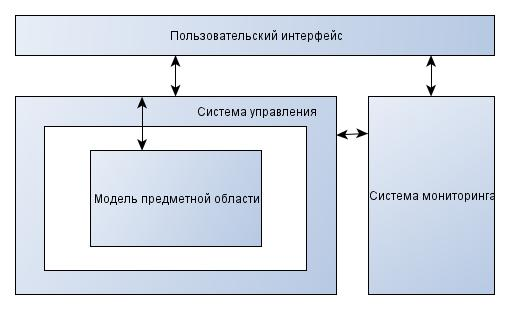
\includegraphics[width = 80mm]{Ch1Pic1}
        \caption{Представление разрабатываемой системы в виде совокупности взаимодействующих компонентов.} \label{Pic1}
    \end{figure}

\section{Выводы}

    Локальная сеть является динамически изменяющейся структурой. Эти изменения связаны с заменой оборудования, добавлением или удалением рабочих станций, смена используемого программного обеспечения и так далее. В некоторых случаях невозможно предусмотреть всех последствий, которые повлечет за собой то или иное изменение, и то может привести к появлению уязвимостей и нарушению безопасности системы. Для сведения к минимуму вероятности таких последствий на этапе разработки сети или в период, предшествующий изменениям, возможно провести испытания по безопасности на модели сети. 

    Моделирование сети позволяет провести исследование различных характеристик процесса функционирования сети, а так же проанализировать различные варианты изменений, которые необходимо внести в структуру сети и выбрать наиболее эффективный. Такой подход позволяет сократить расходы, к которым могут привести ошибочные решения, а так же время, за которое система сможет функционировать в нормальном режиме. 

    Для проведения моделирования сети могут быть использованы различные методы. Наиболее подходящим является метод имитационного моделирования, так как он позволяет изучить поведение системы с различными входными параметрами и проследить динамику изменения системы во времени. Кроме того, построение модели для имитационного моделирования является менее трудоемкой задачей, чем построение математической модели. Для этого могут быть использованы как специально разработанные языки имитационного моделирования, так и языки программирования общего назначения. 

    Для построения модели на языке имитационного моделирования требует от пользователя знания нюансов строения и функционирования различных узлов и протоколов сети, структуры и интенсивности генерации трафика пользователем, владения навыками построения моделей на каком-либо из языков имитационного моделирования. 

    Наиболее эффективным будет использование узкоспециализированной системы моделирования, которая предоставлет возможность пользователь задавать характеристики системы и ее отдельных узлов, при этом модели отдельных компонент предметной области будут включены в состав системы, что позволит в кратчайшие сроки строить модели различной степени сложности. 

    Таким образом, целью дипломного проекта является разработка системы моделирования сетевых атак. Эта система позволит инженеру по безопасности проводить испытания в различных условиях, таких как - нормальный режим и режимы для различных атак. Для достижения этой цели необходимо решить ряд задач:

\begin{itemize}
    \item исследование предметной области, выделение объектов для дальнейшего построения моделей;
    \item разработка моделей объектов и принципа их взаимодействия;
    \item реализация модели объектов с использованием языка программирования общего назначения;
    \item реализация вспомогательных систем, обеспечивающих возможности объединения моделей устройств в модель локальной сети, проведение испытаний, анализ результатов; 
\end{itemize}   

\newpage
\chapter{Построение модели предметной области}
    \section{Описание предметной области}
    \subsection{Описание структуры сети}

    В настоящее время можно выделить несколько типов сетей:
    \begin{itemize}
        \item персональные сети;
        \item локальные сети;
        \item муниципальные сети;
        \item глобальные сети;
    \end{itemize}

    \subsubsection{Персональные сети }

    Персональные сети (PAN) позволяют общаться устройствам вблизи человека. Типичный пример - беспроводная сеть, которая соединяет компьютер с его периферийными устройствами. Почти у каждого компьютера есть присоединенный монитор, клавиатура, мышь и принтер. При отсутствии беспроводной сети они должны быть присоединены кабелями. Примером беспроводной сети может служить беспроводная сеть малой дальности Bluetooth.

    В самой простой форме сети Bluetooth используют парадигму ведущий-ведомые(Master-Slave). Системный модуль (PC) обычно является ведущим устройством и общается с мышью, клавиатурой и.т.д. как с ведомыми устройствами. Ведущее устройство сообщает ведомым какие адреса использовать, когда они могут осуществлять широковещательную передачу, сколько времени они могут передавать, какие частоты использовать и.т.д.

    \subsubsection{Локальные сети}
    Локальными сетями называют частные сети, размещающиеся, как правило, в одном здании или на территории какой-либо организации. Их часто используют для для объединения компьютеров и рабочих станций в офисах компании или предприятия для предоставления совместного доступа к ресурсам и обмена информацией. Беспроводные ЛВС сейчас очень популярны, особенно в домах, более старых офисных зданиях, кафетериях и других местах, где слишком сложно провести кабели.

    Стандарт для беспроводных ЛВС, названный IEEE 802.11, более известный как WiFi, стал очень широко распространен. Он работает на скоростях от 11 до 100 мегабит в секунду.

    В проводных ЛВС используют различные технологии передачи. Большинство из них использует медные провода, а некоторые - оптоволокно. ЛВС ограничены в размере, это означает, что максимальное время передачи ограничено и известно заранее.

    Топология многих проводных сетей создана из магистральных линий. Стандарт IEEE 802.3, обычно называемый Ethernet, является наиболее распространенным типом проводной ЛВС.

    И проводные и беспроводные широковещательные сети в зависсимости от способа назначения канала подразделяются на статические и динамические. При статическом назначении используется циклический алгоритм, и все время делится между всеми машинами на равные интервалы, так что машина может передавать данные только в течении выделенного ей интервала времени. При этом емкость канала расходуется не эффективно, так как временной интервал предоставляется машинам вне зависимости от того, есть ли у них данные для передачи.

    Методы динамического предоставления доступа к каналу так же могут быть централизованными и децентрализованными. При централизованном методе предоставления доступа к каналу должно существовать одно устройство, определяющее машину, получающую право на передачу. Оно должно получать множество пакетов и принимать решение о приоритетах на основании внутреннего алгоритма. При децентрализованном методе каждая машина сама принимает решение о необходимости передачи данных.


    \subsubsection{Муниципальные сети }
    Муниципальные сети (metropolital area network, MAN) объединяет компьютеры в пределах города. Самым распространенным примером муниципальной сети является система кабельного телевидения. В стандарте IEEE 802.16 описана MAN известная всем как WiMax

    \subsubsection{Глобальные сети }

    Глобальные сети (wide area networks, WAN) охватывает значительную географическую область, часто целую страну или даже континент. В состав такой сети входят машины, называемые хостами. Они объединяются в подсети, задача которых - передача трафика от хоста к хосту.

    В большинстве глобальных сетей подсеть состоит из двух раздельных компонентов: линий связи и переключающих компонентов. Линии связи предназначены для передачи данных от машине к машине, в то время как переключающие компоненты необходимы для соединения линий связи. В качестве линий связи используются медный провод, оптоволокно или радиосвязь.

    \subsection{Иерархия протоколов }

    Для упрощения структуры большинство сетей организуется в наборы уровне, каждый последующий является надстройкой над предыдущим. Количество уровней, их название, содержание и назначение разные и зависят от сети. Целью каждого уровня явлется предоставление неких сервисов для вышестоящих уровней. При этом детали реализации остаются скрытыми.

    На рисунке \ref{Pic1} показана пятиуровневая сеть. Взаимодействие между объектами одного уровня не происходит на прямую. Взаимодействующие уровни передают данные нижестоящему протоколу. Так продолжается до самого нижнего уровня. Ниже первого уровня - физическая среда, по которой и происходит обмен информацией.

    \begin{figure}
        \includegraphics[width = 120mm]{Ch2Pic1}
        \caption{Пятиуровневый стек протоколов.} \label{Pic1}
    \end{figure}

    Набор уровней и протоколов называется архитектурой сети. Спецификация архитектуры должна содержать достаточно информации для написания программного обеспечения или создания аппаратуры для каждого уровня, чтобы они корректно выполняли требования протокола. Ни детали реализации, ни спецификация интерфейсов не являются частями архитектуры. При этом не требуется, чтобы интерфейсы на на всех машинах сети были одинаковыми, необходима только корректная обработка данных этими интерфейсами. Список протоколов, используемых системой, по одному протоколу на уровень, называется стеком протоколов.

    \subsection{Эталонные модели взаимодействия}

    \subsubsection{Эталонная модель OSI}

    Эталонная модель OSI(open systems interconnection), за исключение физической среды показана на рисунке \ref{Pic2}. Эта модель имеет семь уровней. Появление именно такой структуры было обусловлено следующими соображениями.
    \begin{itemize}
        \item Уровень должен создаваться по мере необходимости отдельного уровня абстракции.
        \item Каждый уровень должен выполнять строго определенную функцию.
        \item Выбор функций для каждого уровня должен осуществляться с учетом создания стандартизированных международных протоколов.
        \item Границы между уровнями должны выбираться так, чтобы поток данных между интерфейсами был минимальным.
        \item Количество уровней должно быть достаточно большим, чтобы различные функции не объединялись в одном уровне без необходимости, но не слишком высоким, чтобы архитектура не становилась громоздкой.
    \end{itemize}

    \begin{figure}[H]\center
        \includegraphics[width = 140mm]{Ch2Pic2}
        \caption{Эталонная модель взаимодействия открытых систем.} \label{Pic2}
    \end{figure}

    Далее представлено краткое описание каждого уровня рассматриваемой модели.

    \begin{itemize}
        \item Физический уровень. Физический уровень занимается реальной передачей необработанных битов по каналу связи. На данном уровне определяются такие параметры как соответствие напряжения и передаваемого значения, длительность единичного сигнала, направление передачи(дуплекс, полу-дуплекс), начало и окончание передачи сигнала, характеристики канала связи.
        \item Уровень передачи данных. Основная задача -- быть способным передавать "сырые" данные физического уровня по надежной линии связи, свободной от необнаруженных ошибок и маскировать реальные ошибки так, что сетевой уровень их не видит. Эта задача выполняется при помощи разбиения входных данных на кадры,обычный размер которых колеблется от нескольких сот до нескольких тысяч байт.
        \item Сетевой уровень. Сетевой уровень занимается управлением операциями подсети. Важнейшим моментом здесь является определение маршрутов пересылки от источника к пункту назначения. Маршруты могут быть жестко заданы в виде таблиц и редко меняться либо, что бывает чаще, динамически меняться чтобы избегать отказавших компонентов.
        \item Транспортный уровень. Основная функция транспортного уровня - принять данные от сеансового уровня, разбить их при необходимости на небольшие части, передать их сетевому уровню., и гарантировать, что эти части прибудут в правильном виде прибудут по назначению.
        \item Сеансовый уровень. Сеансовый уровень позволяет пользователям различных компьютеров устанавливать сеансы связи друг с другом. При этм предоставляются различные типы сервисов.
        \item Уровень представления. Данный уровень занимается синтаксисом и семантикой передаваемой информации. Чтобы было возможно взаимодействие компьютеров с различным внутренним представлением данных, необходимо преобразовывать форматы данных друг в друга, передавая их по сети в неком стандартизованном виде.
        \item Прикладной уровень. Прикладной уровень содержит набор популярных протоколов, необходимых пользователю.
    \end{itemize}

\subsubsection{Эталонная модель TCP/IP }

    Главной целью возникновения новой архитектуры стало требование объединения различных сетей, для чего от новой архитектуры требовалась гибкость и возможность взаимодействия с существовавшими на тот момент протоколами. Все эти требоания привели к выбору сети с коммутацией пакетов, основанной на уровне без установления соединения, который работает в различных сетях. Рассмотрим уровни, используемые в этой модели (Рисунок \ref{Pic3}).

    \begin{itemize}
        \item Канальный уровень. Данный уровень описывает то, как и что каналы, такие как последовательные линии и классический Ethernet, должны сделать чтобы удовлетворить потребности межсетевого уровня без установления соединения.
        \item Межсетевой уровень. Задача этого уровня заключается в обеспечении возможности каждого хоста посылать пакеты в любую сеть и независимо двигаться к пункту назначения.
        \item Транспортный уровень. Этот уровень создан для того, чтобы объекты одного ранга на приемных и передающих хостах могли поддерживать связь.
        \item Прикладной уровень. Содержит в себе функции сеансового уровня и уровня представления модели OSI, а также пользовательские протоколы высокого уровня.
    \end{itemize}

    \begin{figure}\center
        \includegraphics[width = 120mm]{Ch2Pic3}
        \caption{Эталонная модель TCP/IP.} \label{Pic3}
    \end{figure}

    При разработке модели локальной сети для проектируемой системы будет использована гибридная модель, сочетающая в себе достоинства обоих описанных подходов. Уровни используемой модели показаны на рисунке \ref{Pic4}.

    \begin{figure}\center
        \includegraphics[width = 50mm]{Ch2Pic4}
        \caption{Модель сетевого взаимодействия, используемая при разработке.} \label{Pic4}
    \end{figure}

    \subsection{Сетевые устройства }

    Для обеспечения передачи информации между рабочими станциями, т.е. объединения их в сеть применяются различные устройства. Для удобства их перечисление и описание принципов работы приведено в соответствии используемой моделью сетевого взаимодействия. Для описания процесса взаимодействия между рабочими станциями, необходимо так же описать принцип работы протокола соответствующего уровня.

    \subsubsection{Устройства, взаимодействующие на физическом уровне}

    Физический уровень работы сети связан непосредственно с процессом передачи сигнала. Каждое устройство передачи данных в сети имеет элемент, который преобразует данные в сигнал и передает его. так же это устройство отвечает за прием входящих сигналов.

    Для передачи сигналов от одного передатчика к другому необходим канал связи. При построении локальных сетей используется несколько способов, таких как: беспроводная передача данных и передача данных с использованием соединительных проводов.

    Соединительные провода могут быть разных типов, и обеспечивать различные характеристики передачи сигналов. Например: витая пара, оптоволокно, коаксиальный кабель.

    \subsubsection{Канальный уровень взаимодействия }

    Канальный уровень является логическим уровнем, надстройкой над физическим уровнем. Протокол, работающий на этом уровне решает две основные задачи: контроль среды передачи данных и формирования кадров. Стандарт Ethernet выделяет два подуровня на канальном уровне: MAC и LLC. LLC-подуровень отвечает за формирование кадров и контроль адресов входящих и исходящих передач. MAC(Media Access Control) отвечает за передачу кадров, полученных от LLC-подуровня, через канал связи.

    В случае централизованного контроля передачи данных, проблема разделения среды не возникает. Однако следует рассмотреть вариант децентрализованной передачи, при котором каждая рабочая станция сама принимает решение о необходимости пересылки данных.

    Для примера рассмотрим так называемый классический Ethernet. В качестве среды передачи данных при использовании этого протокола используется так называемая шина -- проводник к которому подключены несколько рабочих станций. Для передачи данных, устройство, контролируемое протоколом MAC-подуровнем "прослушивает" канал связи. В тот момент, когда канал связи является свободным, сетевое устройство начинает передачу данных. При такой реализации возможна проблема одновременного начала передачи несколькими рабочими станциями.

    Для решения такой проблемы используется метод контроля несущей и обнаружения столкновений(CSMA/CD). В случае если в момент исходящей передачи обнаружена входящая, передача прекращается, а в КС посылается jam-последовательность для того, чтобы остальные рабочие станции обнаружили коллизию. Для того, чтобы осуществить передачу и избежать повторной коллизии используется экспоненциальный двоичный алгоритм выдержки, который определяет временную интервал, по истечении которого будет предпринята повторная попытка передачи. Подробнее этот алгоритм будет описан при построении моделей устройств.

    В настоящее время в основном используется коммутируемый Ethernet. Его основное отличие от классического состоит в том, что устройства, объединенные в сеть, подключаются не к общему проводнику, а к устройству, называемому коммутатором(switch). И в случае, если используется дуплексный режим передачи, то коллизий не возникает. Однако, в случае использования полу-дуплексного режима работы, коллизии обрабатываются в соответствии с описанным методом.

    Коммутатор - это устройство, работающее на канальном уровне используемой модели взаимодействия, объединяющее устройства в сеть и отвечающее за пересылку пакетов от отправителя к получателю. Для этого используется таблица коммутации, которая представляет собой соотношение "адрес-порт" и позволяет передавать пакеты не по всей сети а только получателю. при рассмотрении процесса работы коммутатора можно выделить два режима работы.

    \begin{itemize}
        \item режим обучения, во время которого составляется таблица коммутации. Каждому порту ставится в соответствие адрес отправителя, подключенного к этому порту. При этом, если неизвестен порт, к которому подключен получатель, ведется широковещательная рассылка.
        \item Основной режим работы. В этом режиме все пакеты, кроме обозначенных как широковещательные, передаются только получателю.
    \end{itemize}

    \subsubsection{Сетевой уровень взаимодействия }

    Основной задачей, решаемой протоколами сетевого уровня являются задачи маршрутизации пакетов в сети.
    %Возможно стоить добавить общее описание алгоритма маршрутизаци. Хотя он все равно будет в Гл.3.
    Маршрутизатор.

    \subsubsection{Транспортный уровень взаимодействия }

    Конечная цель транспортного уровня заключается в предоставлении эффективных надежных и экономичных услуг(сервисов) передачи данных своим пользователям, которыми обычно являются процессы прикладного уровня. Сервисы транспортного уровня, как и сервисы сетевого уровня, делятся на сервисы с установлением соединения и без установления соединения. Транспортный сервис с установлением соединения во многом похож на аналогичный сервис сетевой сервис. Основным отличием сервисов транспортного уровня является надежность передачи данных.

    \section{Построение моделей }

    \subsection{Общая модель сети. Среда}

        %Общие слова про модель среды, про создание и поддержку существования моделей отдельные объектов.

    Локальная сеть представляет собой соединенные рабочие станции, взаимодействие между которыми осуществляется посредством сетевых протоколов. Общая модель сети является результатом взаимодействия моделей объектов, входящих в ее состав. В связи со сложностью моделирования некоторых процессов, необходимо использовать упрощенные модели. Такими процессами являются например ошибки в каналах связи или процесс генерации пользователем сетевого трафика. Напротив, протоколы взаимодействия представляют собой алгоритмы поведения при обработке данных и, таким образом, представляется возможным создать модели, отражающие это поведение достаточно точно.

    \subsection{Модели устройств}

    Любое устройство, входящее в состав локальной сети взаимодействует с остальными используя соответствующие протоколы. Это позволяет выделить два основных процесса при обмене данными: обработка приема и передачи данных, т.е. непосредственно работа сетевых протоколов, и обработка полученной информации приложением или алгоритмом, в зависимости от устройства, которым данные получены (рисунок \ref{Pic5}).

    \begin{figure}\center
        \includegraphics[width = 60mm]{Ch2Pic5}
        \caption{Общий вид модели устройства.} \label{Pic5}
    \end{figure}

    \subsubsection{Модель канала связи}

    В реальной системе, связанной с передачей данных, всегда существует некоторая вероятность появления ошибки при прохождении сигнала через канал связи. Существует несколько различных моделей каналов связи, обладающих различными характеристиками и по-разному моделирующих ошибку. В рамках разрабатываемой системы используем абстракцию для модели канала связи, обладающую следующими характеристиками:

    \begin{itemize}
        \item доступ к КС может быть получен любым из подключенных устройств в любой момент времени;
        \item передача сигнала всегда происходит с некоторой задержкой;
    \end{itemize}

    Подобная модель позволит строить модель сети с использованием идеального канала связи без помех. Возможность же моделировать ошибку при прохождении сигнала реализуется моделью, которая может входить или не входить в состав представленной.

    \subsubsection{Модель стека сетевых протоколов}

    Модель протокола взаимодействия представляет собой алгоритм обработки данных полученных с нижнего или верхнего уровней. Однако, для правильной организации обмена информацией посредством сети, необходимо объединить используемые протоколы в сеть. Так как разрабатываемая система не подразумевает использование каких-то конкретных протоколов и должна предоставлять возможности для моделирования различных вариантов, то необходимо построить модель абстрактного протокола, при этом реализовав возможность изменения способа обработки данных. Любой протокол предоставляет возможность вышестоящему протоколу отправить данные и принять данные от нижестоящего протокола. Наиболее общая модель протокола представлена на рисунке \ref{Pic6}.
    \begin{figure}\center
        \includegraphics[width = 70mm]{Ch2Pic6}
        \caption{Модель взаимодействия протоколов.} \label{Pic6}
    \end{figure}
    В качестве отдельного типа протоколов можно выделить протоколы, управляющие средой передачи данных. Особенностью таких протоколов является методы контроля за процессом передачи данных, решение возникающих при передаче конфликтов и управления устройством передачи данных. Учитывая эти требования, модель протокола управления средой передачи данных может быть изображена следующим образом(рисунок \ref{Pic7})
    \begin{figure}\center
        \includegraphics[width = 70mm]{Ch2Pic7}
        \caption{Модель взаимодействия стека протоколов со средой.} \label{Pic7}
    \end{figure}
    В некоторых случаях, следует так же выделить в отдельный тип протоколы, используемые на транспортном уровне. В рамках используемой модели взаимодействия, транспортная подсистема представляет собой несколько алгоритмов обработки данных, реализация которых скрыта от пользователя. Для осуществления взаимодействия приложению предоставляется интерфейс, методы которого перечислены в таблице.

    %Сделать нумерацию таблиц.

    \begin{tabular}{|c|c|}
        \hline
        LISTEN & ожидание соединения \\ \hline
        CONNECT & активное установление соединение \\ \hline
        SEND & отправка данных \\ \hline
        RECEIVE & ожидание получения данных \\ \hline
        DISCONNECT & Прервать соединение \\ \hline

    \end{tabular}


    Кроме описанных протоколов, в стеке иногда применяются протоколы для установления соответствия между адресами, используемыми на разных уровнях модели. Такие протокол не связны с приложениями, но связаны с протоколами уровней ниже транспортного. Для адресации на нижних уровнях сети используется MAC-адрес рабочей станции - уникальный идентификатор присваиваемый каждой единице оборудования компьютерных сетей. Но для осуществления взаимодействия между приложениями используются адреса более высоких уровней. Для того, чтобы решить подобную проблему, используют протоколы, которые устанавливают и хранят соответствие между адресами для каждого собеседника. Данный вид взаимодействия изображен на рисунке
    \ref{Pic8}.
    \begin{figure}\center
        \includegraphics[width = 70mm]{Ch2Pic8}
        \caption{Модель взаимодействия служебных протоколов.} \label{Pic8}
    \end{figure}

    Модель любого из описанных протоколов представляет собой конечный автомат. Количество состояний и функции перехода зависят непосредственно от реализации протокола. Так для протоколов сетевого и транспортного уровня с установлением соединения, количество состояний определяется используемыми алгоритмами установления соединений, обмена данными и разрыва соединений.

    Принцип взаимодействия протоколов показан на рисунке \ref{Pic9}.

    \begin{figure}\center
        \includegraphics[width = 120mm]{Ch2Pic9}
        \caption{Пятиуровневый стек протоколов.} \label{Pic9}
    \end{figure}

    \subsection{Моделирование пользовательских процессов}

    Характер сетевого взаимодействия и, следовательно, сетевой трафик, определяется задачами, решаемыми пользователем с использованием рабочей станции и сетевых ресурсов. Оценки характеристик сети передачи данных необходимо иметь возможность моделировать ее поведение в различных ситуациях. Для моделирования нормального режима работы необходимо построить модель генератора трафика, которая будет имитировать нагрузку, близкую по интенсивности и характеру к той, которая генерируется в локальной сети. Моделирование атак различного рода подразумевает подключение к сети злоумышленника, с рабочей станции которого и производится воздействие на компоненты сети. Так же атаки могут быть реализованы с помощью сети интернет, при наличии соответствующего подключения.

    В общем случае пользовательский процесс представляет собой объект, использующий сетевое подключение для обмена информацией с другими процессами. Так как процессы в исследуемой сети рассматриваются с точки зрения оценки нагрузки, то характер передаваемых данных не имеет значения. Поэтому для имитации пользовательской активности используем модели генераторов сетевого трафика, а передаваемые данные будут случайными последовательностями бит.

    Отдельно рассматриваются действия злоумышленника. Для моделирования различного рода атак, пользовательские процессы злоумышленника должны иметь возможность обмениваться "осмысленными" данными с рабочими станциями, и на основе этих данных реализовать имитацию атаки.

    Используемая модель пользовательского процесса представлена на рисунке \ref{Pic10}

    \begin{figure}\center
        \includegraphics[width = 120mm]{Ch2Pic10}
        \caption{Пятиуровневый стек протоколов.} \label{Pic10}
    \end{figure}

    \subsubsection{Модель поведения пользователя}

    Поведение пользователя представлено в модели посредством моделей генерации сетевого трафика. Методы моделирования сетевого трафика можно концептуально разделить на аналитические и имитационные. Аналитическое моделирование подразумевает формальное описание моделируемых объектов и процессов в виде совокупности математических уравнений и выражений. Данные модели удобны для проведения теоретических исследований и формальных манипуляций, однако, в большинстве случаев построение адекватной аналитической модели для многих видов сетевого трафика является практически невыполнимой задачей.

    В том случае, если моделирование ставит перед собой задачу вычисления(оценку) рабочих характеристик параметров моделируемой системы, наиболее предпочтительным является использование имитационных моделей.

    На сегодняшний день можно выделить четыре класса моделей, применяемых для моделирования сетевого трафика:
    \begin{itemize}
        \item использующие классические модели потоков, применяемые в теории массового обслуживания;
        \item основанные на так называемых модулированных случайных процессах;
        \item учитывающие статистическое самоподобие некоторых видов трафика;
        \item строящие имитационные последовательности по образцу трафика.
    \end{itemize}

    Наиболее перспективными на сегодняшний день считаются модели на основе обобщенных модулированных случайных процессов(Generally Modulated Process - GMP) и фрактальные модели на основе хаотических отображений.

    Последние исследования сетей с коммутацией пакетов говорят о статистическом самоподобии некоторых видов трафика и наличии эффекта долгосрочной зависимости.

    Самоподобный трафик обладает следующими статистическими свойствами, важными с точки зрения моделирования:
    \begin{itemize}
        \item распределения временных промежутков поступления пакетов медленно убывают и имеют т.н. "тяжелые хвосты";
        \item распределения временных промежутков поступления пакетов обладают бесконечными моментами(начиная с некоторого порядка);
        \item медленной скоростью ($n_{-1}$) убывания дисперсии вычисленной на основе образца трафика при увеличении длины образца;
    \end{itemize}

    Следует отметить, что в условиях самоподобного трафика классические методы расчета параметров компьютерной сети(пропускной способности каналов, емкости буферов и пр), основанные на пуассоновских потоках, зачастую дают неоправданно оптимистические решения и приводят к недооценки нагрузки.

    Фрактальные модели. Наиболее распространенными моделями, предназначенными для имитации фрактального трафика, являются:

    \begin{itemize}
        \item хаотические отображения;
        \item фрактальное броуновское движение;
        \item фрактальный гауссовский шум;
    \end{itemize}

    Наиболее распространенными и концептуально простыми простыми моделями, позволяющими генерировать самоподобный трафик, являются модели, построенные на так называемый хаотических отображениях(CMAPs). Эти модели используют меньшее число параметров, чем два других метода, и их выбор имеет более наглядную трактовку.

    Одномерное отображение $
        x_{n+1} = \left\{
                    \begin{aligned}
                        f_{1}(n), 0 < x_{n} <= d \\
                        f_{2}(n), d < x_{n} < 1 \\
                    \end{aligned}
                  \right. $
    , где d - параметр отображения называется хаотическим, если функции $f_{1}$ и $f_{2}$ удовлетворяют условию чувствительности к начальным условиям, т.е. расстояние между траекториями через N последовательных итераций можно записать в форме $\|f^{N}(x_{0} + \delta) - f^{N}(x_{0})\| = \delta \cdot e^{N\lambda(x_{0})}$, где $\lambda(x_{0}) > 0$ для большинства значений $x_{0}$.

    Одним из наиболее используемых отображений является последовательность "перемежаемость"

    $$
        x_{n+1} = \left\{
                    \begin{aligned}
                        \epsilon + x_{n} + cx_{m}^{n}, 0 < x_{n} < d, \\
                        \dfrac{x_{n} - d}{1 - d}, d < x_{n} < 1\\
                    \end{aligned}
                  \right.
    $$
    где $c = \dfrac{1 - \epsilon - d}{d_{m}}$.

    Варьируя параметр $\epsilon$ можно изменять продолжительность нахождения модели в первом состоянии, при помощи параметров d и m можно управлять средним значением интенсивности трафика.

    \subsubsection{Построение моделей атак}

    Для моделирования вредоносной активности, рассмотрим два класса атак, применимых в сетях передачи данных.

    В первый класс выделены атаки типа "отказ в обслуживании", спуфинг, т.е. атаки на сетевые протоколы и оборудование. Атаки, принадлежащие к этому классу, ориентированы на протоколы. Для проведения такой атаки, злоумышленник генерирует трафик определенной интенсивности и структуры. Под структурой понимается внутренне строение используемых пакетов. Данный вид атак направлен на использование особенностей работы протоколов в целях получения доступа к передаваемым по сети данным(спуфинг) или повышение интенсивности трафика в сети, что приводит к росту очередей на устройствах обработки данных и снижению производительности сети(атаки типа "отказ в обслуживании"). Таким образом модель представляет собой алгоритм генерации трафика соответствующего назначения.

    Вторым классом атак, рассматриваемых в системе являются атаки на рабочие станции с использованием уязвимостей приложений. Условно процесс атаки на рабочую станцию можно разбить на несколько этапов:

    \begin{itemize}
        \item Сбор информации. Успех атаки напрямую зависит от возможности получить информацию о целевой сети(используемые адреса, операционные системы и доступные сервисы.)
        \item Атака. На этом этапе злоумышленник использует собранную на предыдущем этапе информацию, определяет порядок действий и создает эксплойт. Эксплойт -- это программа, которая внедряет исполняемый код в уязвимую систему.
        \item Сбор информации с использованием доступа к системе. На этом этапе злоумышленник имеет возможности для получения информации, к которой он не имел доступа до компрометации системы.
        \item Повышение привилегий. Используя уязвимости на скопрометированной системе, злоумышленник пытается получить права администратора на локальной машине.
        \item Развертывание. Злоумышленник может использовать доступ к рабочей станции для дальнейшей атаки на другие узлы сети.
        \item Сокрытие следов. На этом этапе злоумышленник скрывает следы свое присутствия в системе.
    \end{itemize}

    Для построения модели ограничимся рассмотрением двух первых этапов атаки: сбор информации и процесс атаки. Модель приложений схематично изображена на рисунке \ref{Pic12}. Каждое приложение представляет собой объект, который может быть использован для атаки атаки на систему. Объекты разделяются на два вида:

    \begin{itemize}
        \item объекты, содержащие уязвимость;
        \item объекты, содержащие информацию, которую можно использовать для эксплуатации уязвимости.
    \end{itemize}


    \begin{figure}\center
        \includegraphics[width = 120mm]{Ch2Pic12}
        \caption{Пятиуровневый стек протоколов.} \label{Pic12}
    \end{figure}

    Модель уязвимости представляет собой вероятностный эксперимент, исход которого зависит от нескольких параметров. Эти параметры разделены на две подгруппы. Первая подгруппа - это характеристики злоумышленника, такие как уровень подготовки, мотив(пен-тест, промышленный шпионаж и.т.д.). Во вторую подгруппу входят параметры, являющиеся информационными. Каждый такой параметр представляет собой информацию, собранную злоумышленником о системе. Данные параметры могут быть как необходимыми для проникновения, так и не влияющими на исход эксперимента. Информация о системе представляется в виде объектов(активов). Эти объекты могут быть получены как путем взаимодействия злоумышленника с целевым сервисом, так и с другими сервисами на рабочей станции, не содержащими уязвимость. Такие сервисы относятся ко второму виду объектов-приложений.

    Второй вид объектов-приложений представлен как модель сервисов, не содержащих уязвимость, но предоставляющих некоторую информацию о системе, которая может быть использована при атаке. Модель такого объекта, как модель объекта, содержащего уязвимость, представляет собой вероятностный эксперимент. Исход этого эксперимента так же зависит от характеристики атакующего.

    В общем виде модель атак, используемая в разрабатываемой системе представляет собой дерево атак(рисунок \ref{Pic13}). Узел $G_{0}$ представляет целевую уязвимость, на которую может быть направлена атака. Каждый узел дерева атаки представляет собой набор промежуточных целей, которые должны быть достигнуты для успешной атаки на главную цель. Промежуточные цели модеут быть представлены в виде И-декомпозиции или ИЛИ-декомпозиции. Цель, представленная ИЛИ-декомпозицией, представляет выбор, при котором должна быть достигнута хотя бы одна из промежуточных целей, для успешной атаки на текущую. Для успеха при атаке на цель, представленную И-декомпозицией, необходимо достижение всех промежуточных целей, которые находятся ниже уровнем.

    \begin{figure}\center
        \includegraphics[width = 120mm]{Ch2Pic13}
        \caption{Пятиуровневый стек протоколов.} \label{Pic13}
    \end{figure}

    Рассматривая пример применительно к используемой модели приложений, следует заметить, что узел $G_{0}$ -- это представление первого вида объектов приложений, т.е. объектов, содержащих уязвимость, а $G_{1}$ ... $G_{6}$ -- это приложения, принадлежащие ко второму виду.

    \subsubsection{Модель поведения злоумышленника}

    Для проведения атаки на компоненты сети передачи данных, злоумышленник должен обладать оборудованием, которое позволит ему совершить провести атаку. Оборудование представляет собой одно или несколько сетевых устройств, чаще всего - рабочих станций, которые имеют доступ в локальную сеть. Оно может быть описано в рамках тех же моделей, которые используются для описания компонентов сети. Главным отличием модели злоумышленника от моделей рабочих станций являются модели приложений. Модель приложений для описания действий злоумышленника включает в себя алгоритм, по которому будет развиваться атака.

   

\section{Выводы}

    На данном этапе работы были разработаны модели устройств, входящих в состав локальной сети. Изучение взаимодействия этих моделей позволит сделать выводы о характере процессов, протекающих в локальной сети, и принять решения о необходимости внесения изменений. 

    На основе построенных моделей необходимо реализовать систему, позволяющую проводить эксперименты над моделью предметной области. Целью данных экспериментов является оценка степени защищенности системы перед определенными классами атак. Учитывая область применения разрабатываемого приложения, пользовательский интерфейс должен быть адаптирован под соответствующие критерии.

    Для реализации системы моделирования необходимо:

    \begin{itemize}
        \item Разработать способ описания используемых при моделировании компонентов.
        \item Реализовать описанные модели компонентов предметной области.
        \item Реализовать систему управления, для создания и контроля параметров модели.
        \item Реализовать систему мониторинга за состоянием объектов. Она включает в себя:
            \begin{itemize}
                \item Сбор информации о состоянии очередей приема и отправки данных на объекте.
                \item Сохранение результатов экспериментов.
                \item Отображение результатов атак на приложения.
            \end{itemize}
    \end{itemize}

    
\newpage

\chapter{Разработка системы моделирования.}
    \section{Разработка архитектуры приложения. }
    Разрабатываемая система позволяет пользователю строить  модель локальной сети, используя объекты, имитирующие поведение различного сетевого оборудования, проводить эксперименты в различных режимах работы, анализировать полученные результаты. Каждая из этих возможностей может быть реализована посредством подсистемы, которые являются компонентами проектируемой системы. Таким образом можно выделить следующие подсистемы.

    \begin{itemize}
        \item Подсистема моделирования. Данная подсистема отвечает за правильное взаимодействие компонентов модели, учитывая их параметры.
        \item Подсистема управления отвечает за сохранение(загрузку) параметров моделей, создание модели сети, а так же предоставляет методы для ее функционирования.
        \item Подсистема мониторинга отвечает за сбор данных в процессе моделирования и их анализ
    \end{itemize}

    \subsection{Подсистема моделирования. }

    Для реализации подсистемы моделирования необходимо описать взаимодействие различных компонент, входящих в ее состав. Такими компонентами являются модели устройств, протоколов, приложений. Объединение сетевых устройств реализовано в проектируемой системе посредством моделей сетевых соединений. Модель локальной сети представляет собой совокупность моделей устройств и их взаимодействия.

    \subsubsection{Канал связи. }

    Для имитации передачи данных могут быть использованы различные модели канала связи. При использовании модели идеального канала без помех единственной характеристикой такого соединения является задержка при передачи данных. В случае необходимости анализа передачи данных в каналах связи с помехами необходима реализация алгоритма генерации помехи. Используемая в системе модель канала связи представлена на рисунке~\ref{Pic2}.

    \begin{figure}[h!]\center
        \includegraphics[width = 60mm]{Ch3Pic2}
        \caption{Диаграмма классов модели канала связи. } \label{Pic2}
    \end{figure}

    Класс NoiseScript описывает алгоритм генерации помехи и связан с моделью канала связи через интерфейс Noise. Такая архитектура позволяет изменять использую модель канала связи без внесения изменений в архитектуру приложения.

    \subsubsection{Протоколы. }

    Для использования при моделировании различных сетевых протоколов они разбиты на четыре группы. К первой группе относятся протоколы, обрабатывающие данные приложений или вышестоящих протоколов. Каждый протокол, относящийся к этой группе, выполняет разделение данных на части и дополняет их служебными полями. В проектируемой модели, использующей стек протоколов TCP/IP, для каждого протокола эти фрагменты данных называются по-разному. Для Ethernet~--~кадры, для IP~--~пакеты, для TCP~--~сегменты. Структура взаимодействия протоколов отражена на рисунке~\ref{Pic3}.

    \begin{figure}[h!]\center
        \includegraphics[width = 40mm]{Ch3Pic3}
        \caption{Диаграмма классов модели протокола. } \label{Pic3}
    \end{figure}

    Анализ служебных полей фрагмента данных описывается в классе, реализующем интерфейс ProtocolScript. Данный механизм позволяет описывать различные протоколы для использования в системе, однако усложняет архитектуру приложения и описание процесса взаимодействия протокола.

    Второй группой протоколов, выделенных на этапе моделирования, являются протоколы управления средой. В стеке протоколов TCP/IP таким протоколом является протокол MAC-подуровня, уровня передачи данных. Отличительной особенностью этих протоколов является связь с устройством передачи данных и возможность контроля за передачей. На рисунке~\ref{Pic4} изображена диаграмма классов, используемая для описания этой группы протоколов.

    \begin{figure}[h!]\center
        \includegraphics[width = 100mm]{Ch3Pic4}
        \caption{Диаграмма классов модели протокола управления средой. } \label{Pic4}
    \end{figure}

    Интерфейс EnviromentControlProtocolScript предоставляет возможность описания различных протоколов управления средой. Для разрабатываемой модели будет реализован метод доступа с контролем несущей и обнаружением коллизий. Данный метод не используется в современных сетях с дуплексным каналом обмена информацией, однако необходим при использовании полудуплексного режима обмена данными.

    Алгоритм, описанный в классе EnviromentControlProtocolScript, определяет возможно ли начать передачу в данный момент времени, возможно ли считать передачу или прием данных успешными и, в некоторых случаях, определяет задержку передачи данных.

    Устройство передачи данных не выполняет никаких действий по контролю за процессом передачи данных, и является моделью передатчика, который генерирует необходимый сигнал и передает его в канал связи.

    Третьей группой протоколов являются служебные протоколы. В стеке протоколов TCP/IP таким протоколом является ARP. Он используется для установления соответствия между физическими адресами и адресами, используемыми на более высоком уровне модели. Для использования этого протокола необходимо внести изменения в архитектуру протоколов первой группы. Для этого добавляется еще один метод для отправки данных, использование которого сопряжено с запросом адреса, используемого на более низком уровне модели, соответствующего адресу на данном уровне. Взаимодействие протоколов первой группы и служебного протокола изображено на рисунке~\ref{Pic5}.

    \begin{figure}[h!]\center
        \includegraphics[width = 100mm]{Ch3Pic5}
        \caption{Схема взаимодействия протоколов передачи данных и служебного протокола. } \label{Pic5}
    \end{figure}

    Протоколы первой и третьей группы являются экземплярами одного и того же класса, который был расширен методами для операций по установлению соответствия адресов. Для подобного рода операций, служебные протоколы связаны с протоколами более низкого уровня, что позволяет им взаимодействовать независимо от адресов более высоких уровней модели.

    К четвертой группе протоколов относятся протоколы, связанные с приложениями. Данный вид протоколов предоставляет приложению интерфейс для обмена данными посредством локальной сети. В рамках используемой модели это протоколы четвертого уровня, содержащие в себе операции транспортного уровня, уровня представления данных и сеансового уровня. Учитывая сложность данных процессов, при реализации протокола TCP было принято решение выделить необходимые операции в отдельную подсистему. Диаграмма классов данной подсистемы представлена на рисунке~\ref{Pic6}.

    \begin{figure}[h!]\center
        \includegraphics[width = 100mm]{Ch3Pic6}
        \caption{Диаграмма классов транспортной подсистемы. } \label{Pic6}
    \end{figure}

    Интерфейс UserTransportFace предоставляет приложению методы для взаимодействия с транспортной подсистемой. Класс ConnectionControlSubsystem отвечает за установление, поддержание и закрытие TCP соединения. В этом классе определяются алгоритмы обработки данных в зависимости от состояния в котором находится соединение. Схема состояний и переходов представлена на рисунке~\ref{Pic7}. На данном уровне абстракции используется понятие сегмента данных. Начальное состояние системы - CLOSED. Управление соединением происходит посредством команд, поступающих от приложения и принятых служебных сегментов.



    \begin{figure}[h!]\center
        \includegraphics[width = 100mm]{Ch3Pic7}
        \caption{Схема конечного автомата TCP-соединения. } \label{Pic7}
    \end{figure}


    Типичный случай клиента, активно соединяющегося с сервером показан на жирными линиями - сплошными для клиента, прерывистыми для сервера. Тонкие линии обозначают необычные последовательности событий. Каждая линия маркирована парой событие/действие. Событие может представлять собой либо обращение пользователя к системной процедуре(CONNECT, LISTEN, SEND или CLOSE), либо прибытие сегмента(SYN, FIN, ACK, RST), либо, в одном случае, окончание периода ожидания, равного двойному времени жизни пакета. Действие может состоять в отправке управляющего сегмента(SYN, FIN или RST). Системные процедуры имеют следующее назначение:
    \begin{itemize}
        \item LISTEN - переводит систему в состояние ожидания соединений.
        \item CONNECT - попытка активного создания соединения.
        \item SEND - отправка данных.
        \item CLOSE - закрытие соединения.
    \end{itemize}

    Управляющие сегменты имеют следующее назначение:

    \begin{itemize}
        \item SYN - сегмент, отправляемый при установлении соединения.
        \item FIN - сегмент, отправляемый при закрытии соединения.
        \item RST - сегмент, отправляемый при сбросе соединения.
        \item ACK - сегмент, отправляемый для подтверждения получения определенного сегмента.
    \end{itemize}

    Назначение того или иного сегмента определяется наличием или отсутствием того или иного флага в TCP-заголовке сегмента.

    Класс SegmentControlSubSystem отвечает за гарантированную доставку сообщений. Это достигается за счет отправки сегмента данных до тех пор, пока не будет получено подтверждение об успешном его приеме.

    \subsubsection{Модели приложений.}

    Приложения, использованные в системе для моделирования действий пользователя, могут использовать протоколы разных уровней. Алгоритмы маршрутизации, используемые в коммутаторах работают на уровне передачи данных, а используемые в маршрутизаторах -- на сетевом уровне, как и алгоритмы генерации трафика. Модели уязвимостей используют транспортную подсистему.

    Приложение, используемое в коммутаторе, представляет собой алгоритм определения соединения, через которое будет направлен полученный пакет. Данный алгоритм имеет два режима работы. Первый - это режим обучения. В этом режиме составляется таблица соответствия физического адреса и порта коммутатора, к которому подключен абонент. При этом полученный пакет передается через все активные порты. Второй режим работы использует построенную на первом этапе таблицу маршрутизации для передачи пакета только указанному получателю. Исключением является широковещательный трафик.

    Построение моделей больших сетей требует использование маршрутизаторов для объединения рабочих станций в подсети и передачи трафика между ними. Приложение, описывающее процесс обработки пакетов, связано с протоколом сетевого уровня используемой модели взаимодействия и является упрощенной реализацией алгоритма маршрутизации. Для определения кратчайшего маршрута при передаче пакета, маршрутизатору необходима информация о состоянии сети и времени передачи пакета тем или иным путем. Для этого используются пакеты состояния линий. Каждый такой пакет содержит информацию об отправителе и "стоимости" пути под ближайших соседей. Для передачи этой информации всем маршрутизаторам в системе  используется алгоритм заливки. Он заключается в том, что каждый маршрутизатор передает полученный пакет на все выходы кроме того, по которому он пришел. Для предотвращения появления в сети большого количества повторных пакетов используется счетчик количества передач, по истечении которого пакет удаляется. Каждый пакет состояния, для определения его актуальности содержит свой порядковый номер. Получая такой пакет, маршрутизатор сверяется с имеющейся у него записью, и если полученный пакет обладает большим порядковым номером, то запись обновляется и пакет пересылается дальше. Если порядковый номер ниже, то пакет отбрасывается. Для сведения к минимуму фактов неверной отбраковки в случае сбоя в счетчике отправителя или ошибки в канале связи, каждый пакет содержит поле "Возраст". Данное поле записывается маршрутизатором и уменьшается на 1 каждую секунду. По истечении счетчика запись удаляется. Имея информацию обо всех маршрутизаторах в сети, для поиска кратчайшего маршрута используется алгоритм Дейкстры.[5]

    Генератор трафика = это приложение, предназначенное для имитации действий пользователя в системе, которые порождают сетевой трафик. На этапе построения моделей, для генераторов трафика было описано хаотическое отображение, описывающее состояние системы. На каждом интервале времени, для системы рассчитывается новое состояние, исходя из которого генерируется соответствующее количество трафика.

    Для моделирования процесса атаки на рабочую станцию, связанного с наличием уязвимости в приложении используем описанную модель активов и уязвимостей. Уязвимость отличается от актива только тем, что в случае удачной атаки, система считается скомпрометированной в то время, как удачная атака на один из активов подразумевает только получение некоторой информации. Для атаки на приложение злоумышленнику необходимо установить TCP-соединение с целевой рабочей станцией и послать соответствующий запрос. Приложение обрабатывает запрос и, с учетом параметров, влияющих на вероятность успеха, либо возвращает некоторую информацию, либо пустое значение, что означает, что атака была неудачной. Диаграмма классов, описывающая взаимодействие моделей приложений и транспортной подсистемы показана на рисунке~\ref{Pic8}

    \begin{figure}[h!]\center
        \includegraphics[width = 100mm]{Ch3Pic8}
        \caption{Диаграмма классов модели пользовательского приложения. } \label{Pic8}
    \end{figure}

    Абстрактный класс Application отвечает за загрузку и передачу данных уязвимостям(Vulnerability) и активам(Asset). Для реализации некоторого приложения, алгоритм его действий необходимо реализовать в классе-наследнике класса Application. На приведенном рисунке таким классом является ListenPortApplication. Данный класс создает TCP-сокет и переводит его в режим ожидания входящего соединения. Подобное поведение наиболее удобно для демонстрации процесса атаки, однако возможна реализация и более сложных алгоритмов.

    Модель поведения злоумышленника так же описывается в классе-наследнике от Application. При этом необходимо описать процесс формирования данных, которые будут отправлены приложению-жертве. В эти данные входит так же и параметры атакующего, такие как мотивация и уровень знаний.

    Каждая модель уязвимости или актива содержит таблицу, в которой хранятся вероятности успеха атаки в зависимости от характеристик атакующего и таблицу необходимой для успешной атаки информации, которая должна содержаться в сообщении злоумышленника.

    Таким образом, диаграмма классов, описывающая структуру модели сетевого устройства может быть изображена следующим образом(рисунок~\ref{Pic9}). Представленное изображение является упрощенным представлением архитектуры модели используемой в приложении. На нем отсутствуют вспомогательные классы, выполняющие различные операции с данными, суть которых не влияет на процесс обработки информации в целом.

    \begin{figure}[pH]\center
        \includegraphics[width = 140mm]{Ch3Pic9}
        \caption{Диаграмма классов модели сетевого устройства. } \label{Pic9}
    \end{figure}

    \subsection{Подсистема управления}

    Подсистема управления обеспечивает создание модели, ее функционирование, и является посредником между моделью и пользовательским интерфейсом, а так же подсистемой моделирования. Создание модели может производится двумя путями. Первый заключается в создании модели с помощью пользовательского интерфейса. При этом, оперируя готовыми моделями устройств и их настройками, возможно создание сетей различных конфигураций. Параметры моделей устройств хранятся в файлах XML, данные в которых разделены по подгруппам. Каждый файл отвечает за объекты, относящиеся к одной группе моделей. Такими группами являются модели приложений, модели стека протоколов, модели устройств. Таким образом модель конечного устройства, которая будет использоваться при моделировании, собирается из разных компонент, за загрузку которых отвечают классы NetworkConfigurationLoader, ApplicationManager. Параметры сетевых устройств, такие как адреса, загружаются классом Network в процессе создания сети. Для связывания данных, хранящихся в XML-файлах и объектов в программе используется набор интерфейсов, который называется JAXB(Java Architecture for XML Binding).

    Класс NetworkConfiguration реализует связывание данных, хранящихся в XML--файле с объектами приложения. По этим данным происходит построение модели модели сети на уровне взаимодействия устройств. Кроме этого, в файле сохраняется информация об используемых в каждом устройстве протоколов и приложений, что позволяет создать модель, описывающую взаимодействие компонентов одного объекта.

    \subsection{Подсистема мониторинга}

    Подсистема мониторинга решает следующие задачи:

    \begin{itemize}
        \item сбор данных, касающихся эффективности работы устройства;
        \item организация и отображение накопленных данных в формате, удобном для дальнейшего анализа;
    \end{itemize}

    Сбор данных в системе реализован посредством системы мониторов. Для этого создается объект-монитор, который сохраняет ссылку на наблюдаемый объект, и с определенной периодичностью снимает необходимые показания. В случае необходимости подсистема сбора данных запрашивает собранные данные и сохраняет их или выводит в форме графиков и таблиц. Взаимодействие компонент подсистемы моделирования представлен на рисунке~\ref{Pic17}

     \begin{figure}[h!]\center
        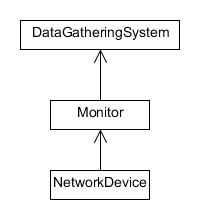
\includegraphics[width = 60mm]{Ch3Pic17}
        \caption{Схема взаимодействия компонент системы мониторинга. } \label{Pic17}
    \end{figure}

    Для оценки проблемы доступности данных, одним из наблюдаемых параметров является состояние очереди обработки пакетов сетевого устройства. Данный параметр непосредственно влияет на скорость реакции сервера, в случае поступления к нему запроса. Поэтому, для оценки этого параметра система моделирования позволяет вывести график, иллюстрирующий состояние очереди в каждый момент времени.

    Еще одной возможностью системы моделирования является проведение тестов на проникновение. Исход каждой попытки сохраняется в системе мониторинга отдельно для каждого устройства и при необходимости может быть проанализирован пользователем. Так же в эту таблицу для каждого устройства заносятся факты превышения определенной длины очереди обработки пакетов. Эта ситуация может свидетельствовать как о неправильной конфигурации устройства или неэффективной конфигурации сети, так и об атаке на отказ в обслуживании.



    \section{Описание работы приложения}

    \subsection{Создание модели}

    Для создания модели исследуемой сети предусмотрено несколько возможностей. Во-первых -- создание файла-конфигурации сети, с описанием всех устройств и соединений. При этом описание каждого устройства должно содержать список протоколов, которые используются устройством,  список приложений, с упоминанием используемых классов, описывающих действия приложения, уникальные идентификаторы устройства и адреса используемые в сетевом взаимодействии. Второй возможностью является использование пользовательского интерфейса. Данный интерфейс реализует механизмы, позволяющие пользователю создавать устройства с минимальными настройками, после чего проводить дополнительную конфигурацию в случае необходимости. Вид пользовательского интерфейса программы представлен на рисунке~\ref{Pic10}.

    \begin{figure}[h!]\center
        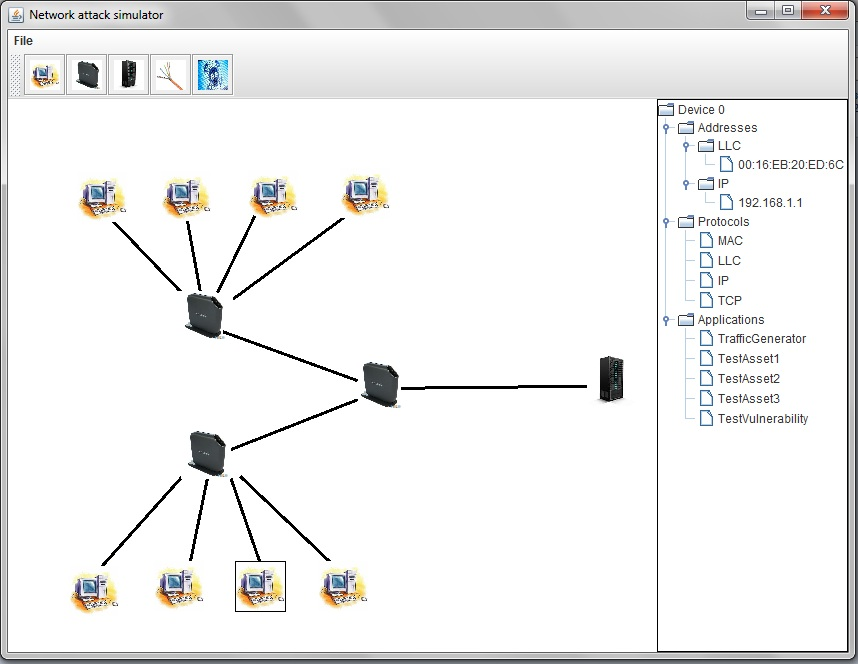
\includegraphics[width = 100mm]{SystemMainView}
        \caption{Диаграмма классов модели пользовательского приложения. } \label{Pic10}
    \end{figure}

    Главное меню приложения состоит из двух пунктов: File и Simulate. Меню File предоставляет функции по сохранению и загрузке различных моделей. Меню Simulate реализует возможности по управлению моделью и просмотру статистики по проведенным экспериментам.

    Панель, расположенная под главным меню, содержит кнопки для создания примитивов модели. Подсистема моделирования различает только два вида объектов - объекты-устройства и объекты-соединения. Различия устройств в характере обработки информации проявляются во внутренней конфигурации и используемых приложениях. Пользовательский интерфейс устанавливает дополнительные различия для удобства использования и, соответственно, задает устройствам различные начальные конфигурации. Объект "рабочая станция" представляет собой модель рабочей станции внутри локальной сети. Используемый стек протоколов - TCP/IP. В системе моделирования не рассматриваются различные виды трафика и протоколы, работающие выше транспортного уровня, поэтому единственным приложением, используемым по умолчанию является генератор трафика, который использует хаотическую функцию, описанную во второй главе. Объект "Сервер" отличается от объекта "рабочей станции" использованием в качестве приложения модели обработки входящего трафика и так же использует генератор трафика с иными параметрами хаотической функции. Каждое из описанных устройств имеет по одному сетевому порту. Объект "маршрутизатор" использует протоколы трех уровней модели взаимодействия: физического, передачи данных и сетевого, при этом с сетевым уровнем непосредственно взаимодействует алгоритм маршрутизации, реализованный как приложение низкого уровня. Маршрутизатор "по умолчанию" имеет 10 портов. Объект "Злоумышленник" по исходной конфигурации не отличается от рабочей станции и выделен в отдельную категорию для удобства управления его конфигурацией и поведением. Исходной конфигурацией объекта "соединение" является канал связи без помех.

    При выделении устройства открывается дерево его свойств, с помощью которого возможно изменить различные параметры устройства, добавить или удалить те или иные приложения и протоколы, однако, существует вероятность удаления необходимого для работы устройства компонента. В этом случае, некоторая часть модели может работать некорректно, что в свою очередь ведет к искажению результатов эксперимента.

    Для просмотра состояния какого либо из объектов предусмотрено использование контекстного меню, появляющегося при выделении устройства и щелчке правой кнопкой мыши. Это меню представлено на рисунке~\ref{Pic11}.

    \begin{figure}[h!]\center
        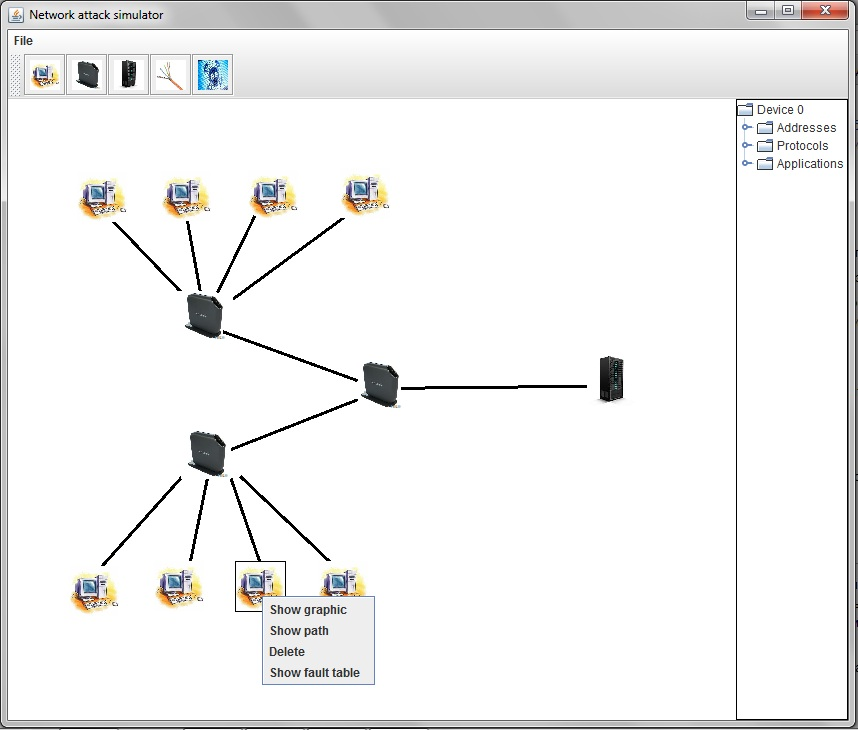
\includegraphics[width = 100mm]{contextMenuView}
        \caption{Диаграмма классов модели пользовательского приложения. } \label{Pic11}
    \end{figure}

    \subsection{Использование функций приложения}

    Для наглядности описания пользовательского интерфейса и возможностей программы, рассмотрим модель небольшой сети, состоящей из двух подсетей, объединяющих рабочие станции,  и сервера приложений. Исследуемой характеристикой в данном случае является состояние очереди обработки пакетов на сервере приложений, так как от нее зависит скорость, с которой пользователь может получить интересующие его данные. Для просмотра статистики по состоянию очереди необходимо вызвать пункт меню "Show graphic". Результат этой операции представлен на рисунке~\ref{Pic12}.

    \begin{figure}[h!]\center
        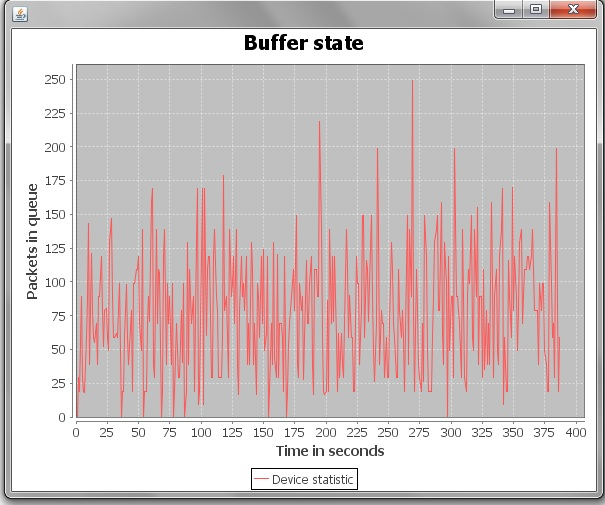
\includegraphics[width = 100mm]{LoadGraphic}
        \caption{График состояния очереди сервера. } \label{Pic12}
    \end{figure}

    На этом графике изображен размер очереди в различные моменты времени от начала моделирования. Для данного примера можно сделать вывод о том, что установка размера очереди в 1000 КБайт будет вполне достаточно для работы сети в нормальных условиях. Однако, манипуляции с интенсивностью трафика изменяют эту картину. Кроме количества пакетов в очереди, еще одной важной характеристикой является вид графика. На рисунке~\ref{Pic12} представлен график нормальной работы сервера, при
    которой он справляется с нагрузкой. Рассмотрим случай повышенной интенсивности трафика(рисунок~\ref{Pic13}).

    \begin{figure}[h!]\center
        \includegraphics[width = 100mm]{LoadGraphicOverload}
        \caption{График состояния очереди сервера. Перегрузка. } \label{Pic13}
    \end{figure}

    В данном случае график имеет вид неубывающей кривой, что сигнализирует о том, что сервер не справляется с генерируемой нагрузкой и в некоторый момент времени, независимо от максимального размера очереди возникнет перегрузка. В случае, если описанное поведение не является режимом DDos атаки, но является моделированием обычного режима, необходимо проверить параметры генераторов трафика устройств в сети и, если они адекватно описывают процесс генерации реального трафика в исследуемой сети, то необходимо пересмотреть конфигурацию сервера и, возможно, использовать более производительное оборудование.

    Еще одной возможностью программы является просмотр маршрутов трафика, связанного с некоторым объектом сети. Данная возможность включается в контекстом меню устройства, пункт "show path". При включении данной опции, каждое соединение, по которому проходит пакет с адресом получателя или отправителя эквивалентного адресу устройства, для которого задействована эта функция.

    На рисунке~\ref{Pic14} представлено использование этой функции для рассматриваемого примера. В данном случае, соединения, по которым проходит пакет с наблюдаемым адресом в поле отправитель окрашены в зеленый(\#00ff00) цвет, а поле получатель -- в голубой(\#00ffff). Эта опция позволяет отследить маршруты трафика для устройства и смоделировать возможности перехвата и перенаправления трафика.


    \begin{figure}[h!]\center
        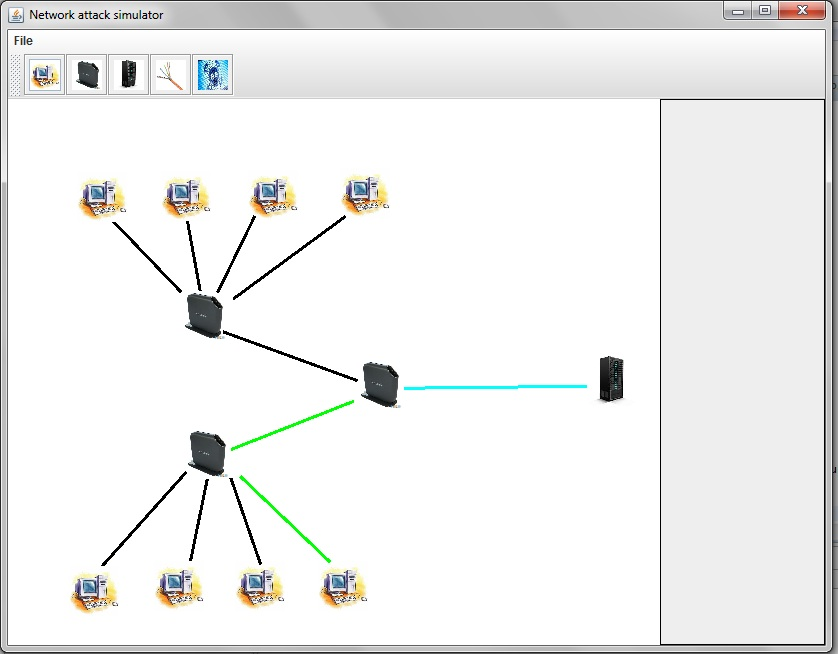
\includegraphics[width = 100mm]{routing}
        \caption{Маршруты пересылки пакетов для выбранного устройства. } \label{Pic14}
    \end{figure}

    Моделирование атак на проникновение не отображается на рассмотренном представлении модели и может быть проанализировано только посредством таблиц, в которых хранятся данные об атаках. Для этого используется пункт меню "show faults table". Faults table или таблица неисправностей представляет собой записи обо всех случаях, угрожающих нормальной работе устройства. Кроме рассматриваемых тестов в эту таблицу так же попадают записи о перегрузках в очереди устройства. В случае, если таблица неисправностей не пуста, устройство, которому она принадлежит приобретает рамку, окрашенную в красный цвет, которая отображается в независимости от того выделено устройство или нет(рисунок~\ref{Pic15}).


    \begin{figure}[h!]\center
        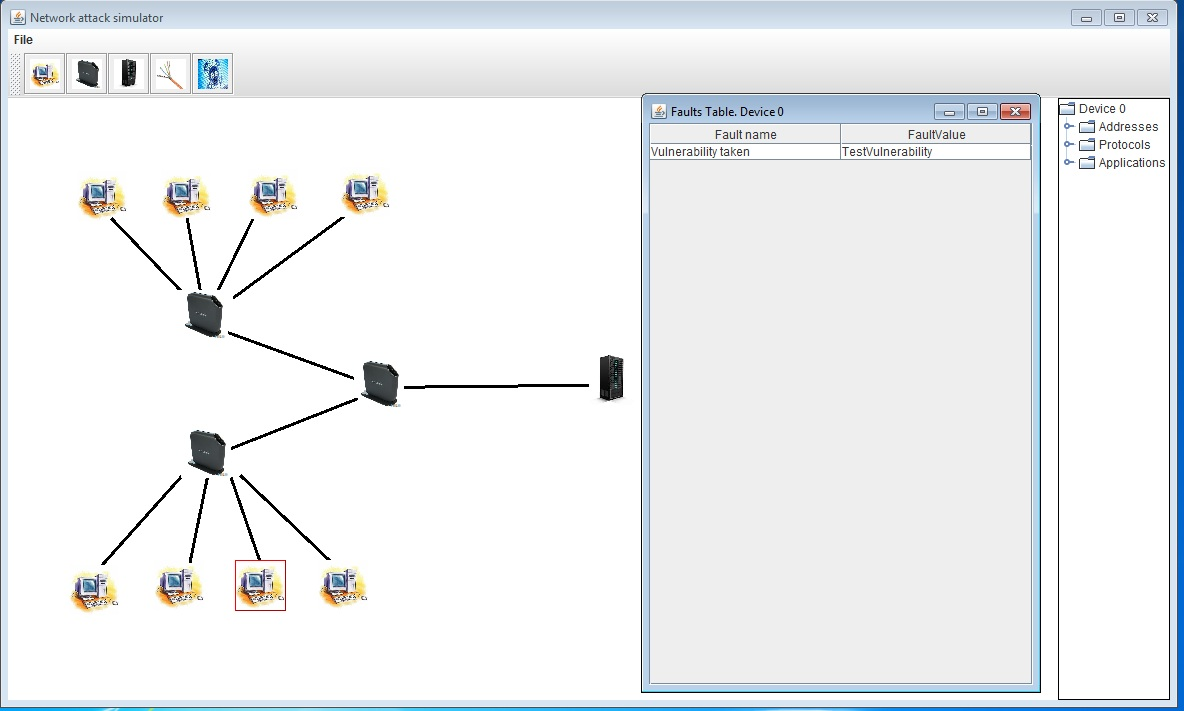
\includegraphics[width = 100mm]{FaultsTable}
        \caption{Таблица неисправностей для выбранного устройства. } \label{Pic15}
    \end{figure}

    Для рассматриваемого примера таблица неисправностей состоит из одной записи, что говорит о том, что имеющаяся в конфигурации устройства уязвимость была эксплуатирована злоумышленником. Однако по результатам одного теста нельзя говорить о степени защищенности той или иной сети или устройства в сети. Используемая модель проведения атак не гарантирует точного ответа на этот вопрос.

    Выводы о степени защищенности исследуемой системы можно сделать по результатам серии испытаний, для чего в меню "Simulate" выделен пункт "Statistics". На рисунке~\ref{Pic16} изображена такая таблица для семи испытаний. Эта таблица во многом повторяет значения таблицы неисправностей, но хранит эти значения для всех экспериментов, проведенных с моделью. По данным этой таблицы можно, при достаточном их количестве, можно провести статистическую оценку степени угрозы, которую представляет та или иная уязвимость.

    \begin{figure}[h!]\center
        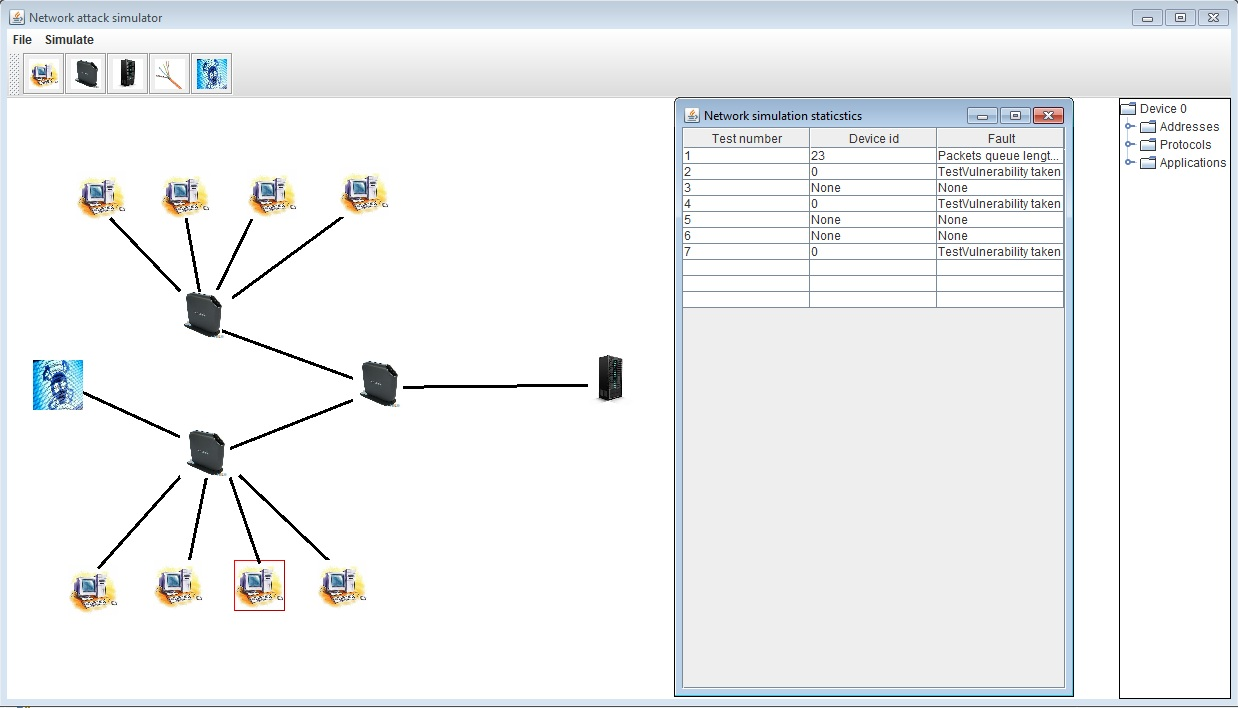
\includegraphics[width = 100mm]{StatisticsTable}
        \caption{Таблица результатов серии экспериментов. } \label{Pic16}
    \end{figure}

    \subsection{Анализ производительности}

    Рассмотренный пример является лишь способом описания возможностей системы и не является примером ее реального использования. Для сетей такого размера обычно не применяют методов моделирования, так как все неисправности, касающиеся производительности сети можно устранить в кратчайшие сроки. Методы имитационного моделирования используются в сетях с десятками и сотнями рабочих станций, организованных в подсети.

    Проведенный анализ показал возможность использования данной системы для моделирования средних и больших локальных сетей. Данные по анализу представлены в таблице~\ref{table1}
    \begin{table}[h!]
        \caption{Затраты вычислительных ресурсов ЭВМ при моделировании сетей различного размера}\label{table1}
        \begin{tabular}{|c|c|c|}

            \hline
            Количество устройств & Загрузка процессора & Используемая память(Мбайт) \\ \hline
            100 & 3\% & 260 \\ \hline
            200 & 5\% & 450 \\ \hline
            300 & 7\% & 610 \\ \hline

        \end{tabular}
    \end{table}

    Моделирование производилось на ЭВМ со следующими параметрами:

    \begin{itemize}
        \item Процессор Intel Pentium P6000 1.87GHz (2-ядра);
        \item Оперативная память 4Гб.
    \end{itemize}

    \subsection{Выводы}

    На данном этапе проектирования системы была реализована модель предметной области, описанная во второй главе, а так же другие компоненты системы моделирования, необходимые для проведения экспериментов. Реализованная модель предметной области представляет собой совокупность объектов, и процесса их взаимодействия. Каждый объект в свою очередь так же может быть разбит на несколько более мелких, реализующих те или иные его функции.

    Реализованная система позволяет проводить эксперименты, необходимы для оценки безопасности передачи данных в локальной сети, а также эффективность принимаемых мер по повышению защищенности. Несмотря на то, что некоторые возможности предоставляются пользователю готовыми к использованию, от него требуется наличие минимальных навыков по конфигурации сети, а так же знание о методах статистического анализа данных. При этом программа спроектирована таким образом, чтобы пользователь имел возможность внесения изменений в некоторые ее части, а именно, в файлы, описывающие алгоритмы поведения различных систем. В большей степени это касается алгоритмов приложений. Пользователь системы, обладая необходимыми навыками в программировании, может написать собственные модели приложений, отвечающие необходимым требованиям и более точно отражающие поведение используемых приложений и оборудования.

    Данная система может на ЭВМ различной мощности, так как не требует большого количества ресурсов, что показал проведенный анализ производительности. Однако моделирование больших вычислительных сетей может потребовать использования ЭВМ с большим объемом оперативной памяти. 

\newpage

\chapter{Экономическая оценка}
\section{Концепция экономической оценки}


В современном мире невозможно представить себе область деятельности, в которой не используются средства вычислительной техники. Процесс обработки информации с использованием таких средств, становится в большей степени автоматизированным, что позволяет значительно увеличить эффективность работы. Для обеспечения удобного обмена данными между локальными рабочими станциями, передачи данных в хранилище и.т.д. их необходимо объединить в сеть.  При этом обрабатываемые данные могут быть различной степени конфиденциальности, кроме того, вопросы целостности и доступности имеют большое значение в процессе эффективного функционирования организации. Однако, объединение средств вычислительной техники в сети открывает некоторые возможности для злоумышленника получить доступ к данным или  иным способом нарушить информационный обмен между рабочими станциями.

Нарушение нормальной работоспособности сети может повлечь за собой неприемлемые для организации последствия. Например, фирма может потерять прибыль из-за нарушения конфиденциальности данных или неспособности оказать услугу в данный момент времени, из-за нарушения стабильной работы сервера.
Для сокращения риска возникновения подобных ситуаций, организации используют различные средства защиты. Это могут быть как аппаратные средства, такие как, например,  межсетевые экраны, программные средства, такие как антивирусы, системы анализа трафика или комплексные решения, например, системы обнаружения вторжения.

Эффективность использования упомянутых средств зависит не только от их качества, но и от правильного их использования, что является задачей инженера по безопасности. Однако сложность правильного использования средств защиты напрямую зависит от сложности сети. В случае больших сетей, которые имеют место в крупных организациях, упомянутая сложность становится не только угрозой безопасности, но проблемой неэффективного использования финансовых средств.
Для проведения предварительного анализа и выявления возможных проблем используются различные системы моделирования. Существуют системы, решающие проблему доступности данных, т.е. позволяющих построить в заданных условиях наиболее быстро функционирующую сеть. Другие системы, такие как сканеры уязвимостей, позволяют выявлять наличие мест, в которых потенциально возможна успешная атака на защищаемые данные. Некоторые системы позволяют оценить возможность той или иной атаки на сеть.

Темой дипломного проекта является: "Разработка системы моделирования атак на вычислительную сеть". Разрабатываемая система обладает рядом преимуществ:
\begin{enumerate}
\item возможность оценки вероятности компрометации какой-либо системы в составе локальной сети.
\item возможность оценки состояния сети при атаках типа "отказ в обслуживании".
\item удобный пользовательский интерфейс.
\end{enumerate}

Данная система позволяет инженеру по безопасности провести моделирование различных режимов функционирования сети, в т.ч.  режимы атаки, и по результатам тестирования принять решение о необходимости использования тех или иных средств защиты или изменения конфигурации сети. Разрабатываемая система объединяет в себе возможности моделирования потоков сетевого трафика и возможностей по эксплуатации уязвимостей. Таким образом, данная система позволяет уменьшить риски при работе с конфиденциальной информацией.

Данная разработка является независимой и автономной.

Разрабатываемая система может быть применена при проектировании архитектуры крупных вычислительных сетей с целью анализа состояний объектов, участвующих в информационном обмене и выявлении возможных точек образования очередей и неисправностей.

Экономическое обоснование не производится, а производится ее оценка, т.к. на данном этапе НИР отсутствует информация о результатах применения.

Экономическая оценка эффективности проводимой в дипломном проекте научно-исследовательской работы направлена на доказательство актуальности тематики, а также на оценку научно-технического уровня полученных результатов. Экономическая оценка работы будет состоять из следующих разделов:

\begin{enumerate}
\item трудоемкость выполнения НИР.
\item смета затрат на проведение НИР
\item экономическая оценка эффективности НИР
\end{enumerate}

Выполнение дипломной работы проходило на базе Санкт-Петербургского государственного электротехнического университета. 

\section{Трудоемкость выполнения НИР}
В данном разделе рассмотрим перечень основных этапов и видов работ, которые должны быть выполнены для достижения целей НИР.

Данные по трудоемкости и срокам выполнения НИР приведены в таблице~\ref{table1}.

Исполнителями НИР являются старший научный сотрудник и студент-выпускник высшего учебного заведения (инженер). Учитывая эти данные, была определена трудоемкость выполняемых работ.

\begin{table}
\caption{Трудоемкость и сроки выполнения НИР.}\label{table1}
\begin{tabular}{|p{1em}|p{15em}|p{7em}|p{6em}|p{8em}|}
  \hline
  № & Наименование работ & \multicolumn{2}{|c|}{Трудоемкость, чел/дни} & Машинное время маш/час \\
  \ & \ & Старший научный сотрудник & Инженер & \ \\ \hline
  1 & Постановка задачи и утверждение ТЗ. & 1 & 1 & - \\ \hline
  2 & Сбор информации по существующим решениям и анализ полученных данных & - & 5 & 30 \\ \hline
  3 & Анализ научных работ в исследуемой области & - & 5 & 20 \\ \hline
  4 & Анализ методов моделирования. & - & 5 & 30  \\ \hline
  5 & Формулировка технического задания  & 1 & 1 & - \\ \hline
  6 & Разработка моделей устройств для системы  & 2 & 10 & 60 \\ \hline
  7 & Разработка архитектуры приложения & 2 & 10 & 60  \\ \hline
  8 & Реализация системы & 1 & 20 & 150  \\ \hline
  9 & Анализ и оценка разработанной системы & 1 & 1 & 5 \\ \hline
  10 & Исправление ошибок & - & 5 & 30  \\ \hline
  11 & Составление и оформление отчета по НИР & - & 10 & 40 \\ \hline
  12 & Сдача проекта & 1 & 1 & - \\ \hline
  \multicolumn{2}{|r|}{ИТОГО:} & 9 & 73 & 435 \\ \hline
\end{tabular}
\end{table}

\section{Смета затрат на проведение НИР}
В этом разделе мы оценим затраты, необходимые на проведение НИР. Основными статьями калькуляции являются материалы, спецоборудование, расходы на оплату труда, отчисления на социальные нужды, прочие прямые расходы и накладные расходы.

\subsubsection{Статья "Материалы"}

К статье "Материалы" отнесем расходы, представленные в таблице~\ref{table2}.

\begin{table}[h!]\center
\caption{Расходы на материалы}\label{table2}
\begin{tabular}{|p{10em}|p{10em}|p{9em}|p{9em}|}
  \hline
  Наименование товара & Количество & Стоимость за единицу, руб & Стоимость, руб \\ \hline
  Картридж для принтера & 1 & 2500 & 2500 \\ \hline
  Бумага А4 & 1 пачка & 150 & 150 \\ \hline
  Канцелярские принадлежности & 1 комплект & 100 & 100 \\ \hline
  \multicolumn{3}{|c|}{Итого} & 2750 \\ \hline
  \multicolumn{3}{|c|}{Транспортно-заготовительные расходы(15\%)} & 410 \\ \hline
  \multicolumn{3}{|c|}{Итого} & 3160 \\ \hline
\end{tabular}
\end{table}

\subsubsection{Статья "Спецоборудование"}
  Расходы на данную статью не предусмотрены.

\subsubsection{Статья "Расходы на оплату труда"}

Данные по статье "Расходы на оплату труда" представлены в таблице~\ref{table3}.
\begin{table}[h!]
\caption{Расходы на оплату труда}\label{table3}
\begin{tabular}{|p{12em}|p{10em}|p{9em}|p{7em}|}
  \hline
  Участник НИР & Зар.плата за месяц & Количество рабочих дней & Общая сумма \\ \hline
  Старший научный сотрудник & 40000 & 9 & 19200 \\ \hline
  Инженер & 25000 & 73 & 97300 \\ \hline
  \multicolumn{3}{|c|}{Итого} & 116500 \\ \hline
\end{tabular}
\end{table}

Основная заработная плата исполнителей рассчитывается по формуле:

\begin{center}
$C_{ЗО} = \dfrac{T_{1} \cdot C_{ЗОмес}}{t} \cdot (1 + \dfrac{H_{H}}{100})$
\end{center}

где $T_{1}$ -- трудоемкость выполнения работ руководителя и инженера.

    $C_{\text{ЗОмес}}$ -- месячные оклады исполнителей.

    $H_{H}$ -- норматив начислений, 12\%

    $t$ -- среднее количество рабочих дней в месяце(21).

\subsubsection{Статья "Страховые взносы в государственные внебюджетные фонды"}

Ставка социального налога составляет 30\%, включающие в себя отчисления в:

\begin{enumerate}
  \item Пенсионный фонд Российской Федерации -- 22\%
  \item Фонд Социального страхования Российской Федерации -- 2,9\%
  \item Федеральный фонд обязательного медицинского страхования -- 2,1\%

\end{enumerate}
Таким образом налог составляет:

  $C_{\text{CH}} = C_{\text{ЗО}} \cdot \dfrac{H_{CH}}{100}$

  $C_{\text{CH}} = 116500 \cdot \dfrac{30}{100} = 34950$

\subsubsection{Статья "Затраты по работам, выполненным сторонними организациями"}

В качестве расходов на оплату услуг сторонних организаций условно выступает стоимость машинного времени.

Стоимость машинного времени рассчитывается по формуле:

\begin{center}
$C_{\text{МВ}} = t_{\text{МВ}} \cdot P_{\text{МВ}}$
\end{center}

где:

$t_{\text{МВ}}$ -- время использования ПЭВМ(435 часов)

$P_{\text{МВ}}$ -- стоимость машиннго часа времени (условно 30 руб/час)

$C_{\text{МВ}} = 435 \cdot 30 = 13050$ руб.

\subsubsection{Статья "Командировочные расходы"}
Затраты на служебные командировки не предусмотрены.

\subsubsection{Статья "Прочие прямые расходы"}

К статье "прочие прямые расходы" относятся расходы на получение специальной научно-технической информации, за использование средств связи и коммуникации и другие расходы, необходимые для проведения НИР.

В таблице~\ref{table4} представлены статьи, относящиеся к прочим прямым расходам.

\begin{center}
\begin{table}\center
\caption{Прочие прямые расходы}\label{table4}
\begin{tabular}{|c|c|}
  \hline
  Наименование & Сумма, руб. \\ \hline
  Internet & 300 \\ \hline
  Книги & 1500  \\ \hline
  Другие расходы &  216 \\ \hline
  Итого & 2016\\ \hline
\end{tabular}
\end{table}


$C_{\text{ПР}} = C \cdot k$

$C_{\text{ПР}} = 1800 \cdot 1,12$ = 2016

\end{center}

где k -- коэффициент учитывающий другие виды прочих прямых расходов.

\subsubsection*{Статья "Накладные расходы"}

В статью "накладные расходы" мы включим все расходы на управление и хозяйственное обслуживание. Так как в период проведения НИР в работе оборудования не было никаких сбоев, то затраты, связанные с его ремонтом не учитываем. Величина накладных расходов определяется на основании норматива, установленного в СПбГЭТУ, и берется равной 33\%.

\begin{center}
$C_{\text{НР}} = C_{\text{ЗО}} \cdot \frac{H_{HP}}{100}$

$C_{\text{НР}} = 116500 \cdot \frac{33}{100} = 38445$
\end{center}

\subsubsection*{Статья "Себестоимость НТПр"}
В таблице~\ref{table5} представлены все основные статьи калькуляции расходов, необходимых для проведения НИР.

Себестоимость рассчитывается по формуле:

$C = C_{M} + C_{\text{ЗО}} + C_{CH} + C_{\text{МВ}} + C_{\text{ППР}} + C_{HP} = 208121$

\begin{table}[h!]
\caption{Себестоимость НТПр}\label{table5}
\begin{tabular}{|c|c|}
  \hline
  Статья затрат & Сумма, руб \\ \hline
  Материалы & 3160 \\ \hline
  Спецоборудование &  - \\ \hline
  Расходы на оплату труда & 116500\\ \hline
  Страховые взносы в государственные внебюджетные фонды & 34950\\ \hline
  Затраты по работам, выполненным сторонними организациями & 13050\\ \hline
  Командировочные расходы & - \\ \hline
  Прочие прямые расходы & 2016\\ \hline
  Накладные расходы & 38445\\ \hline
  Итого Себестоимость & 208121\\ \hline
\end{tabular}
\end{table}

\textbf{Итого общая стоимость разработки составляет $C_{o} = 208121$ руб.}

\section{Комплексная оценка эффективности НИР.}

В данной разработке производится качественная оценка экономической эффективности НИР. Это объясняется этапом выполнения НИР, а также отсутствием на данном этапе информации о применении разработки и возможности ее сбыта, потому оценка экономической эффективности НИР включает качественную оценку эффекта от разработки и научно-технические уровни (уровень качества) выполненной разработки.

Количественная оценка экономической эффективности НИР отсутствует, в связи с тем, что на данном этапе отсутствует информация о результатах применения разработки.

Разработанная система предназначена для решения ряда задач, в том числе таких, для решение которых не предусмотрено в иных программных комплексах, близких по назначению к данной системе.  Произведем оценку уровня качества в сравнение с системой Cisco Packet Tracer(П1)(таблица~\ref{table6}).

\begin{table}[h!]
\caption{Сравнение характеристик конкурирующей разработки} \label{table6} 
\begin{tabular}{|p{1em}|p{17em}|p{4em}|p{7em}|p{7em}|}
  \hline
  № & Характеристики & \multicolumn{2}{|c|}{Оценка в бальной шкале} & Коэффициент значимости $\alpha_{i}$ \\
  \ & \ & П1 & Разработанная система & \ \\ \hline
  1 & Моделирование стандартного режима & 9 & 8 & 0,3 \\ \hline
  2 & Моделирование критического режима(атака на отказ в обслуживании) & 9 & 8 & 0,4 \\ \hline
  3 & Моделирование атаки на проникновение & 2 & 5 & 0,2 \\ \hline
  4 & Пользовательский интерфейс & 8 & 8 & 0,1 \\ \hline
\end{tabular}
\end{table}

Уровень качества вычисляется по формуле:

\begin{center}
  $K_{\text{кач}} = \sum_{i=1}^n \alpha_{i} \cdot \dfrac{\text{Б}_{i}}{\text{Б}_{\text{баз}}} \approx 1,22$
\end{center}

Расчет эффективности НИР:

\begin{center}
  $\text{Э}_{\text{НИР}} = \dfrac{C_{O}}{K_{\text{кач}} \cdot 100\%} = \dfrac{208121}{122} = 1706  \text{руб}/\%$
\end{center}

Это означает, что для того, чтобы повысить уровень качества на один процент было затрачено 1706 руб.

Кроме того, следует отметить, что разработанная система позволяет уменьшить риски при обработке важной информации, что в конечном итоге приведет к снижению издержек и потерь пользователя.

Все вышеизложенное показывает экономическую целесообразность разработки НТПр.

\subsection*{Выводы}

По результатам проведенной экономической оценки, можно сделать следующие выводы:

\begin{enumerate}
  \item Трудоемкость НТПр составляет 73 чел/дней для инженера и 9чел/дней для старшего научного сотрудника.
  \item Себестоимость НТПр составляет 208121 руб.
  \item Уровень качества НТПр составляет 1,22
\end{enumerate}

К сожалению отсутствие информации не позволяет провести оценку экономической эффективности, но высокий технический уровень решения делает научную разработку эффективной.


\newpage
\chapter{Охрана интеллектуальной собственности}

    В ходе выполнения дипломного проекта мною, Андриановым Кириллом Сергеевичем, была разработана программа для ЭВМ "Система моделирования сетевых атак". Этот результат научно-технической деятельности входит в перечень охраняемых объектов интеллектуальной собственности Гражданского кодекса РФ. Программа разработана по личной инициативе , права на программу принадлежат автору - Андрианову Кириллу Сергеевичу, так как программа разработана в рамках учебного процесса.

    Под интеллектуальной собственностью понимают особый вид гражданских прав (исключительное право) в отношении результатов интеллектуальной деятельности, таких как изобретения, промышленные образцы (дизайн), компьютерные программы, другие произведения науки, произведения литературы, искусства, которые принято называть объектами интеллектуальной собственности, а также различных средств индивидуализации производителя товаров и услуг, таких как товарные знаки, знаки обслуживания, фирменные наименования и др. [2, ст. 1225]. Основным содержанием таких прав является монополия их владельца на использование этих объектов, включая право запретить или разрешить их использование другим, а также право переуступить другому лицу эти правомочия или отказаться от них вовсе.

    Согласно определению интеллектуальной собственности, принятому в российском законодательстве, а также на основании определения Стокгольмской конференции от 14 июля 1967 г., программы для ЭВМ (компьютерные программы) и базы данных относятся к объектам интеллектуальной собственности. Программам для ЭВМ и базам данных предоставляется охрана нормами авторского права как литературным произведениям в соответствии с Бернской конвенцией, причем программы для ЭВМ \
    охраняются как литературные произведения, а базы данных - как сборники.

    В Российской Федерации вопросы предоставления правовой охраны программам для ЭВМ и базам данных регулируются Гражданским кодексом РФ, Часть 4 (ГК РФ Ч.4).

    Под программой для ЭВМ понимается "... представленная в объективной форме совокупность данных и команд, предназначенных для функционирования ЭВМ и других компьютерных устройств в целях получения определенного результата". Кроме того, в понятие программы для ЭВМ входят "...подготовительные материалы, полученные в ходе разработки программы для ЭВМ, и порождаемые ею аудиовизуальные отображения" [2, ст. 1261].

    С точки зрения программистов и пользователей программа для ЭВМ представляет собой детализацию алгоритма решения какой-либо задачи и выражена в форме определенной последовательности предписаний, обеспечивающих выполнение компьютером преобразования исходных данных в искомый результат. Можно выделить следующие объективные формы представления программы для ЭВМ:

    \begin{itemize}
        \item исходная программа (или исходный текст) - последовательность предписаний на алгоритмическом (понятном человеку) языке высокого уровня, предназначенных для автоматизированного перевода этих предписаний в последовательность команд в объектном коде;
        \item рабочая программа (или объектный код) - последовательность машинных команд, т. е. команд, представленных на языке, понятном ЭВМ;
        \item программа, временно введенная в память ЭВМ, - совокупность физических состояний элементов памяти запоминающего устройства ЭВМ (ОЗУ), сохраняющихся до прекращения подачи электропитания к ЭВМ;
        \item программа, постоянно хранимая в памяти ЭВМ, - представленная на языке машины команда (или серия команд), выполненная в виде физических особенностей участка интегральной схемы, сохраняющихся независимо от подачи электропитания.
    \end{itemize}

    Исходная и рабочая программы, как правило, представляются в виде записи на том или ином языке, выполненной на бумаге или машиночитаемом носителе данных: магнитном или оптическом диске, магнитной ленте и т. п.

    Предоставляемая законодательством правовая охрана распространяется "... на все виды программ для ЭВМ (в том числе на операционные системы и программные комплексы), которые могут быть выражены на любом языке и в любой форме, включая исходный текст и объектный код …" [2, ст.1261]. Так как преобразование исходного текста программы для ЭВМ в объектный (машинный) код с помощью специальных программ-трансляторов не меняет сущности данной программы как произведения, то если охраняется исходный текст программы, значит, охране подлежит и соответствующий ей объектный код. Обратное тоже справедливо.

    Правовая охрана программ для ЭВМ распространяется только в отношении формы их выражения и "… не распространяется на идеи, концепции, принципы, методы, процессы, системы, способы, решения технических, организационных или иных задач, открытия, факты, языки программирования" [2, ст.1259, п. 5].

    Предпосылкой охраноспособности программы для ЭВМ и базы данных является их творческий характер, т. е. они должны быть продуктом личного творчества автора. Творческий характер деятельности автора предполагается до тех пор, пока не доказано обратное [2, ст. 1257].

    Момент возникновения авторского права является важнейшим юридическим фактом, который устанавливается в силу создания произведения (программы для ЭВМ или базы данных). "Для возникновения, осуществления и защиты авторских прав не требуется регистрация произведения или соблюдение каких-либо иных формальностей" [2, ст.1259, п.4].

    Часто возникает вопрос: насколько необходимо для возникновения прав на программу для ЭВМ или базу данных их обнародование? Закон устанавливает, что это не является обязательным условием: "Авторские права распространяется как на обнародованные, так и на необнародованные произведения, выраженные в какой-либо объективной форме …" [2, ст. 1259, п. 3].

    Таким образом, только сам факт создания программы или базы данных, зафиксированных в объективной форме, является основанием возникновения авторского права на эти объекты. С этого момента права автора или иного правообладателя защищаются законом.

    Права в отношении программ для ЭВМ и баз данных подразделяются на личные неимущественные и исключительные права.

    Личные права включают право авторства, право на имя и право на неприкосновенность (целостность), право на обнародование программы для ЭВМ или базы данных [2, ст. 1265-1268]. Они связаны непосредственно с автором программы для ЭВМ или базы данных: принадлежат лицу, чьим творческим трудом созданы программа для ЭВМ или база данных - автору, являются неотчуждаемыми, т. е. не могут быть переуступлены другому лицу, и не ограничены каким-либо сроком [2, ст. 1228].

    Исключительные права непосредственно связаны с понятием "использования" программ для ЭВМ и баз данных: "Автору произведения или иному правообладателю принадлежит исключительное право использовать произведение … в любой форме и любым не противоречащим закону способом …" [2, ст. 1270, п.1]. При этом под использованием понимается осуществление определенных действий с программами для ЭВМ или базами данных, а именно: опубликование (выпуск в свет); воспроизведение (полное или частичное) в любой форме, любыми способами; распространение; модификацию и иное использование [2, ст. 1270, п.2]. Они могут принадлежать автору или иному правообладателю (гражданину или юридическому лицу). Правообладатель может распоряжаться исключительным правом на произведение [2, ст. 1270, п.1], в том числе по своему усмотрению разрешать или запрещать другим лицам использование [2, ст. 1229, п.1]. Распоряжение принадлежащим правообладателю исключительным правом может осуществляться любым, не противоречащим закону и существу такого исключительного права способом, в том числе путем его отчуждения по договору другому лицу или предоставления другому лицу права использования [2, ст. 1233, п.1]. Срок действия исключительного права ограничен

    Каждая составляющая понятия использования программы для ЭВМ или базы данных имеет конкретное содержание, которое также определено законом:
    \begin{itemize}
        \item   воспроизведение - "... изготовление одного или более экземпляров произведения или его части в любой материальной форме, … в том числе запись в память ЭВМ" [2, ст. 1270, п. 2, п.п.1];
        \item распространение - предоставление доступа к произведению "... путем продажи или иного отчуждения его оригинала или экземпляров" [2, ст. 1270, п. 2, п.п.2].
        \item публичный показ (выпуск в свет) - "... любая демонстрация оригинала или экземпляров произведения непосредственно … … либо с помощью технических средств в месте, открытом для свободного посещения, или в месте, где присутствует значительное число лиц … " [2, ст. 1270, п. 2, п.п.3];
    \end{itemize}

    Обращает на себя внимание то, что понятие "использование" не связано с функционированием программы (или ее выполнением) с целью получения результата. Последнее лучше относить к понятию "потребление" или "пользование" программы. Поэтому каждый раз, когда пользователь запускает программу для того, чтобы произвести расчеты, построить графики или таблицы и т. п., он не "использует" (поскольку не создается новый экземпляр), а "потребляет" программу, не нарушая при этом ничьих прав.

    В целях оповещения о своих правах правообладатель "... вправе использовать знак охраны авторского права, который помещается на каждом экземпляре произведения и состоит из следующих элементов: латинской буквы С в окружности; имени или наименования правообладателя; года первого опубликования произведения" [2, ст. 1271]. Знак охраны авторского права может проставляться на упаковке, на самом программном продукте, а также на всех сопроводительных и дополнительных материалах, однако это не является обязательным. Следует иметь в виду, что сам знак ничего не защищает (защищает закон!), и что наличие или отсутствие знака охраны никак не связано с возникновением авторского права. Знак охраны авторского права - это цивилизованная форма предупреждения желающих использовать данный объект, что права на него охраняются законом, с одновременным сообщением о том, кому эти права принадлежат.

    Исключительные права на программу или базу данных переходят по наследству в установленном законом порядке, и их можно реализовать в течение срока действия авторского права.

    Права на программу для ЭВМ или базу данных не связаны с правом собственности на материальный носитель, на котором они зафиксированы. Передача прав на материальный носитель не влечет за собой передачи каких-либо прав на программу для ЭВМ или базу данных [2, ст.1227]. Иными словами, передача носителя информации (например, дискеты) с зафиксированной на нем программой третьему лицу не означает передачи каких-либо прав на эту программу.

    
    \newpage
    \thispagestyle{empty}
    \ \\
    \ \\
    \ \\
    \ \\
    \ \\
    \ \\
    \ \\
    \ \\
    \ \\

    \begin{center}

        \textbf{ПРОГРАММА ДЛЯ ЭВМ.}

        \large\textbf{Система моделирования сетевых атак.}

        Фрагменты исходного текста программы.
        
        120 стр.
    \end{center}

    \ \\
    \ \\
    \ \\
    \ \\
    \ \\
    \ \\
    \ \\
    \ \\
    \ \\



    Правообладатель: Андрианов Кирилл Сергеевич.

    Автор: Андрианов Кирилл Сергеевич.
    \ \\
    \ \\
    \ \\
    \ \\
    \ \\
    \ \\


    \copyright Андрианов К.С., 2013.


    \ \\
    \ \\
    \ \\


    \begin{center}
        Санкт-Петербург

        2013
    \end{center}

\newpage

    \begin{center}
        \large\textbf{ СОСТАВ ПРОГРАММНОГО КОМПЛЕКСА.}
    \end{center}

    Каталог bin.
    \begin{itemize}
        \item каталог Main
        \begin{itemize}
            \item каталог Devices
            \begin{itemize}
                \item NetworkDeviceConfiguration -- хранение характеристик модели сетевого компонента.
            \end{itemize}
            \item каталог managers
            \begin{itemize}
                \item ApplicationsManager -- хранение характеристик моделей приложений.
                \item ThreadPoolManager -- управление потоками в процессе моделирования.
            \end{itemize}
            \item каталог model
            \begin{itemize}
                        \item каталог scripts -- хранятся объекты, описывающие частное поведение моделей приложений
                        \item Application -- объект, описывающий общее поведение моделей приложений
                        \item LowLevelApplication -- интерфейс, декларирующий методы взаимодействия с моделями протоколов сетевого уровня.
                        \item Vulnerability -- интерфейс, декларирующий методы, используемые в модели уязвимости.
                        \item NetworkConnection -- объект, являющийся моделью физического соединения(Канала связи).
                        \item Transmitter -- объект, являющийся моделью устройства, генерирующего и принимающего сигналы по каналу связи.
                               \item ByteQueue -- очередь байт для отправки или обработки получения.
                               \item ConnectionControlSubSystem -- объект-модель системы контроля соединения в протоколе TCP.
                               \item ConnectionConfiguration -- объект, сохраняющий параметры соединения.
                               \item SegmentControlSubSystem -- объект, реализующий соединение, управляющий передачей пакетов.
                               \item TCPSegment -- объект, описывающий структуру данных, используемую в протоколе TCP.
                        \item DataRepresentationSystem -- объект, преобразующий данные их формы, используемой в приложении в форму, используемую в протоколе.
                        \item TCPSocket -- объект, используемый для обеспечения взаимодействия между приложением и протоколами передачи данных.
                \item Generator -- объект, являющийся моделью для имитации сетевого трафика, создаваемого пользователем.
                \item Network -- объект, являющийся верхним уровнем модели сети и используемый для кофигурирования и управления глобальными параметрами модели.
                \item NetworkDevice -- объект, являющийся моделью устройства, участвующего в сетевом взаимодействии.
            \end{itemize}
            \item каталог protocols
                \begin{itemize}
                    \item каталог scipts -- в нем содержатся файлы, описывающие реализацию конкретного протокола.
                    \item AbstractProtocol -- класс, описывающий общее для всех протоколов операции.
                    \item EnviromentProtocol -- класс описывающий действия для протоколов управления средой передачи данных.
                    \item ProtocolScript -- интерфейс, декларирующий методы, используемые в протоколе.
                    \item ProtocolStack -- объект, объединяющий протоколы, для управления и конфигурации.
                \end{itemize}
            \item каталог subsystems
                \begin{itemize}
                    \item NetworkConfigurationLoader -- объект, который считывает и хранит конфигурацию модели.
                \end{itemize}
        \end{itemize}
        \item Config -- объект, хранящий глобальные переменные для процесса моделирования.
        \item Main -- точка входа в программу и запуск необходимых подсистем.
    \end{itemize}

    Каталог data

    \begin{itemize}
        \item application\_description.xml -- файл, в котором хранятся настройки моделей приложений.
        \item network\_devices\_confguration.xml -- файл, в котором хранятся настройки моделей сетевых устройств.
        \item protocol\_stacks.xml -- файл, в котором хранятся настройки моделей сетевых протоколов.
    \end{itemize}


    \subsubsection{Реферат.}

    \begin{tabular}{p{15em}p{25em}}
        Автор: & Андрианов Кирилл Сергеевич \\
        Правобладатель: & Андрианов Кирилл Сергеевич \\
        Программа для ЭВМ: & Система моделирования сетевых атак \\
        Аннотация : & Система предназначена для моделирования процесса атак на вычислительную сеть. Система реализована таким образом, что каждый ее отдельный компонент может быть модернизирован без ущерба для остальных частей программы. Модернизация может включать в себя как изменение работы алгоритма, уже существующего, так и создание нового, описывающего иную модель поведения объекта, отличную от рассмотренных. Программа позволяет строить модели сетей различной структуры и оценивать их работоспособность и эффективность в различных условиях. Так же в программе существует возможность моделирования атаки на отдельные рабочие станции. Данная возможность осуществляется с помощью моделей приложений и моделей уязвимостей. Эта модель представляет собой вероятностный эксперимент, результатом которого является успех или неудача. \\

        Тип ЭВМ: & IBM PC-совместимый компьютер. \\
        ОС : & Любая. Необходима JAVA-машина версии не ниже 6.\\
        Язык программирования : & JAVA. \\
        Объем : & 246 Кбайт.
    \end{tabular}

\newpage

\begin{center}
    ЛИЦЕНЗИОННЫЙ ДОГОВОР

    НА ИСПОЛЬЗОВАНИЕ ПРОГРАММЫ ДЛЯ ЭВМ
\end{center}

    Стороны в Договоре:

    Гражданин Андрианов Кирилл Сергеевич, проживающий по адресу: 198320, г. Санкт-Петербург, Гатчинское шоссе, д. 13, корп.1 кв. 6, именуемый в дальнейшем "ЛИЦЕНЗИАР", с одной стороны, и Государственное образовательное учреждение высшего профессионально-го образования "Санкт-Петербургский государственный электротехнический университет "ЛЭТИ" им. В.И.Ульянова (Ленина)", именуемый в дальнейшем "ЛИЦЕНЗИАТ", в лице проректора по научной работе Шестопалова М.Ю., действующего на основании Доверенности, с другой стороны, принимая во внимание:
\begin{enumerate}
    \item что Лицензиар является автором и правообладателем программы для ЭВМ "Система моделирования сетевых атак";
    \item Лицензиат желает получить на условиях настоящего Договора лицензию на ис-пользование упомянутой программы для ЭВМ с целью проведения научных ис-следований в области медицинского приборостроения;
    \item Лицензиар готов предоставить Лицензиату такую лицензию, договорились о следующем.
\end{enumerate}

\begin{enumerate}
    \item Термины и их определения
    \begin{enumerate}
        \item "ПРОГРАММА ДЛЯ ЭВМ (ПрЭВМ)" - программное обеспечение "Система моделирования сетевых атак".
        \item "ДОКУМЕНТАЦИЯ" - комплект документов, передаваемых Лицензиаром Лицензиату, включающий руководство пользователя по применению и обслуживанию программы для ЭВМ.
        \item "ПРОИЗВОДСТВЕННАЯ ПЛОЩАДКА" - научные лаборатории и кафедры Лицензиата.
        \item "РАБОЧЕЕ МЕСТО" - конкретная ЭВМ, на которой используется Программа для ЭВМ.
    \end{enumerate}
    \item Предмет Договора
        \begin{enumerate}
            \item Лицензиар предоставляет Лицензиату на срок действия настоящего Договора и за вознаграждение, уплачиваемое Лицензиатом, неисключительную лицензию на использование ПрЭВМ. При этом Лицензиату предоставляется право на установку ПрЭВМ не более чем на 10 (десяти) Рабочих местах.
            \item Лицензиар передает Лицензиату Документацию к ПрЭВМ.
            \item Предоставленное Лицензиату в рамках настоящего Договора право ограничено Производственной площадкой.
            \item Лицензиар осуществляет авторский контроль за соблюдением объемов ис-пользования ПрЭВМ по настоящему Договору, при этом Лицензиат обеспечивает возможность такого контроля.
            \item Лицензиар сохраняет за собой право самому использовать ПрЭВМ и предоставлять неисключительные лицензии на право ее использования третьим лицам.
        \end{enumerate}
    \item Обеспечение Договора
    \begin{enumerate}
        \item Лицензиар передает Лицензиату ПрЭВМ в объеме и виде, достаточном для ее использования, и Документацию в течение 15 (пятнадцати) дней со дня подписания настоящего Договора. ПрЭВМ передается Лицензиату в виде   в количестве 5 (пяти) штук, содержащих ПрЭВМ. По факту передачи ПрЭВМ и Документации составляется акт сдачи-приемки с перечнем переданных материалов, подписываемый обеими Сторонами.
        \item Если Лицензиат установит неполноту или неправильность полученных ПрЭВМ или Документации, то Лицензиар в течение 15 (пятнадцати) дней после сообщения ему об этом Лицензиатом обязан передать недостающие материалы или устранить недостатки ранее переданных ПрЭВМ и Документации.
        \item Для оказания помощи в освоении ПрЭВМ Лицензиар по просьбе Лицензиата оказывает консультации пользователям ПрЭВМ.
        \item Для целей использования ПрЭВМ в объеме, предусмотренном п. 2.1 настоящего Договора, Лицензиат может изготавливать в необходимом ему количестве копии ПрЭВМ и копии Документации.
    \end{enumerate}
    \item Усовершенствования.
    \begin{enumerate}
        \item Лицензиар обязуется незамедлительно информировать Лицензиата о всех произведенных им усовершенствованиях ПрЭВМ и, при желании Лицензиата, передать ему в согласованные сроки новые варианты ПрЭВМ. В отношении новых вариантов ПрЭВМ, переданных Лицензиаром Лицензиату, распространяются все условия настоящего Договора.
        \item Лицензиат обязуется предоставлять Лицензиару информацию об использовании ПрЭВМ, которая могла бы быть полезной для усовершенствования ПрЭВМ.
    \end{enumerate}
    \item Платежи.
    \begin{enumerate}
        \item За предоставление прав, предусмотренных настоящим Договором, Лицензиат выплачивает Лицензиару единовременное вознаграждение в размере 20000(двадцать тысяч) рублей.
        \item Вознаграждение, предусмотренное п. 5.1 настоящего Договора, выплачивается Лицензиатом в течение 30 (тридцати) дней, следующих после подписания акта приемки-сдачи.
    \end{enumerate}
    \item Реклама
    \begin{enumerate}
        \item Лицензиат обязуется при опубликовании результатов исследований, полученных с использованием ПрЭВМ, сообщать в рекламных целях, что исследования производились с использованием ПрЭВМ Лицензиара с указанием авторского права Лицензиара.
    \end{enumerate}
    \item Защита передаваемых прав
    \begin{enumerate}
        \item Лицензиат обязуется не вносить самовольно каких-либо изменений в ПрЭВМ и Документацию и не дополнять их какими-либо комментариями. Подобные изменения или дополнения возможны только с согласия Лицензиара.
        \item Лицензиат обязуется предпринимать все необходимые меры для предотвращения несанкционированного копирования ПрЭВМ и Документации третьими лицами, а также несанкционированной передачи ПрЭВМ и Документации работниками Лицензиата третьим лицам.
        \item Если Лицензиату станет известно о противоправном использовании ПрЭВМ третьими лицами, то он незамедлительно сообщит об этом Лицензиару.
    \end{enumerate}
    \item Ответственность Сторон и разрешение споров.
    \begin{enumerate}
        \item За невыполнение или ненадлежащее выполнение обязательств по настоящему Договору Стороны несут имущественную ответственность в соответствии с действующим законодательством.
        \item Стороны освобождаются от ответственности за неисполнение или ненадлежащее исполнение обязательств, принятых по настоящему Договору, если неисполнение явилось следствием обстоятельств непреодолимой силы (форс-мажор).
        \item Сторона, нарушившая свои обязательства по настоящему Договору, освобождается от ответственности за неисполнение или ненадлежащее исполнение этих обязательств, если это нарушение было вызвано причинами, за которые отвечает другая Сторона.
        \item В случае возникновения споров между Лицензиаром и Лицензиатом по вопросам, предусмотренным настоящим Договором, Стороны примут все меры к разрешению их путем переговоров между собой. В случае невозможности разрешения указанных споров путем переговоров они будут разрешаться в порядке, предусмотренном действующим законодательством.
    \end{enumerate}
    \item Срок действия Договора и условия его расторжения
    \begin{enumerate}
        \item Настоящий Договор заключен на срок 2 года и вступает в силу с даты его подписания обеими Сторонами.
        \item По истечении срока действия настоящего Договора Лицензиат вправе использовать ПрЭВМ, включая усовершенствованные варианты, на Производственной площадке на любом количестве Рабочих мест. При этом обязательства Лицензиата, предусмотренные пп. 7.1 и 7.2 настоящего Договора, сохраняются бессрочно.
        \item Действие настоящего Договора по обоюдному согласию Сторон может быть досрочно прекращено, но не ранее чем через три месяца после предложения об этом одной из Сторон. При этом Лицензиат не освобождается от обязательств по платежам, возникшим до расторжения настоящего Договора.
        \item Настоящий Договор может быть досрочно расторгнут в одностороннем порядке со стороны Лицензиара из-за невыполнения Лицензиатом своих обязательств по пп. 7.1 или 7.2. В этом случае Лицензиат лишается права дальнейшего использования ПрЭВМ в любой форме и обязан вернуть ее Лицензиару.
        \item Если Лицензиат откажется от дальнейшего использования ПрЭВМ, то он уничтожит все имеющиеся у него копии ПрЭВМ.
    \end{enumerate}
    \item Заключительные положения.
    \begin{enumerate}
        \item Все изменения и дополнения к настоящему Договору действительны только в тех случаях, если они совершены в письменной форме и подписаны обеими Сторонами.
        \item Стороны не имеют права передавать свои права и обязательства по на-стоящему Договору третьим лицам без письменного согласия на то другой Стороны.
        \item Во всем остальном, что не предусмотрено условиями настоящего Договора, будут применяться нормы законодательства Российской Федерации.
    \end{enumerate}
    \item Адреса Сторон
    \begin{enumerate}
        \item ЛИЦЕНЗИАР: Андрианов Кирилл   Сергеевич, адрес: 198320, Санкт-Петербург, Гатчинское шоссе д.13,  корп.1, кв.6.
        \item ЛИЦЕНЗИАТ: СПбГЭТУ, адрес: 197376, Санкт-Петербург, ул. Проф. Попова, д. 5.
    \end{enumerate}
\end{enumerate}

Настоящий Договор составлен в двух экземплярах для каждой из Сторон и подписан "\underline{\ \ \ }"\underline{\ \ \ \ \ \ \ \ \ \ } 200\underline{\ \ } г. в г. Санкт-Петербурге.
\\
\\

\begin{tabular}{p{20em}p{20em}}
    ЛИЦЕНЗИАР: &   От ЛИЦЕНЗИАТА: \\
     & Проректор по научной работе СПбГЭТУ \\
    \underline{\ \ \ \ \ \ \ \ \ \ \ }  К.С. Андрианов & 	

            \underline{\ \ \ \ \ \ \ \ \ \ \ \ } В.М. Кутузов
            \\
\end{tabular}

\newpage 
\chapter*{Заключение}

   Целью данного дипломного проекта являлась реализация системы моделирования атак на вычислительную сеть. В процессе проектирования было проведено исследование существующих языков имитационного моделирования для использования их в качестве возможных альтернатив созданию новой системы. Описанные средства моделирования являются непригодными для использования в рамках поставленной задачи, так как обладают высоким уровнем абстракции, относительно предметной области, и требуют специальных знаний и навыков в области моделирования, в то время как разрабатываемая система ориентирована на использование инженером по безопасности. 
   
   В связи с этим было решено использовать язык программирования общего назначения JAVA. В связи с разнородностью объектов, входящих в состав предметной области, было использовано несколько подходов к построению моделей, а именно: модель детерминированного конечного автомата, математические модели, описывающие генерацию трафика. Рассматривая предметную область как совокупность независимых компонентов и процесса их взаимодействия, были реализованы отдельные части моделей, которые могут быть использованы пользователем для построения собственных моделей. 
   
   Реализованная система обладает возможностями анализа загруженности сетевых узлов, маршрутов трафика, а так же возможностью проведения тестов на проникновение. Каждая из этих возможностей позволяет моделировать атаки различного рода, оценивать степень защищенности системы и эффективность мер, принимаемых для повышения уровня безопасности. 
   
   Одним из главных требований к разрабатываемой системе была гибкость, то есть возможность использования различных моделей поведения для устройств, изменение и добавление новых моделей без внесения крупных изменений в исходный код приложения. Реализацией этого требования стали классы, описывающие поведение моделей устройств и приложений. Соответствие между устройством и используемым приложением устанавливается в конфигурационном файле и является уникальным для каждого устройства.
   
    Таким образом можно сделать вывод, что поставленные задачи решены полностью. 
    
    Экономическая оценка результатов НТПр, выполненная в ходе проектирования имеет следующие показатели:
    
    \begin{itemize}
        \item Трудоемкость НТПр составляет 73 чел.дней для инженера и 9 чел.дней для руководителя.
        \item Себестоимость НТПр составляет 208121 руб.
        \item Уровень качества НТПр составляет 1.22.
    \end{itemize}

    \subsubsection{Перспективы развития системы}
    
    В ходе дипломного проектирования была создана система, позволяющая проводить эксперименты с моделью локальной сети. Данные, полученные в результате тестов, сохраняются в подсистеме сбора данных. Для принятия решения относительно уровня безопасности системы и мер, которые возможно принять для его повышения, данные, полученные в ходе экспериментов необходимо проанализировать и по результатам анализа вынести соответствующее решение. В связи с этим дальнейшим развитием данной системы, для использования в ходе проектирования локальной сети, является реализация модуля статистического анализа данных и системы поддержки принятия решений, которая генерирует рекомендации по улучшению уровня безопасности локальной сети.

\newpage

\chapter*{Список использованной литературы}

\renewcommand{\labelenumi}{\arabic{enumi}.}

\begin{enumerate}
    \item Советов Б.Я., Яковлев С.А., Моделирование систем –М.:Высш.Шк., 2001.

    \item Stefan Karpinski Realistic model of local network traffic, 2005.

    \item Добровольский Е.В., Нечипорук О.Л., Моделирование сетевого трафика с использование контекстных методов, 2005.

    \item  Leland W.E., Taqqu M.S. Willinger W., Wilson D.V. On the self-similar nature of ethernet traffic, 1994.

    \item Таненбаум Э., Уэзеролл Д., Компьютерные сети –Спб.:Питер, 2012.

    \item  Gorodetsk V., Kotenko I., Attacks against computer network: Formal grammar-based framework and simulation tool, 2002.

    \item  Lye K., Wing J. Game strategies in network security, 2005.

    \item  Kumar S., Spafford E.H. An application of pattern matching in intrusion detection, 1994.

    \item Гудов А.М., Семехина М.В., Имитационное моделирование процессов передачи трафика в вычислительных сетях.

    \item Шенон Р., Имитационное моделирование систем. Искусство и наука.

    \item Степашкин М.В., Котенко И.В., Богданов В.С., Моделирование атак для активного анализа уязвимостей компьютерных сетей.

    \item  Ingols K., Chu M.,Lippmann R., Webster S., Boyer S.,  Modeling modern network attacks and and contermeasures using attack graphs, 2009.

    \item  Kotenko I., Stepashkin M., Ulanov A. Agent-based modeling and simulation of malefactors attacks against computer networks, 2006.

    \item  Lathrop S. D., Hill J., Surdu J.R.,  modeling network attacks.

    \item  Sarraute C., Fernando Miranda, Jose I. Orlicki, Simulation of computer networks.

    \item  Goldman R.P., Stochastic model for intrusions, 2002.

    \item  Liu P., Zang W., Incentive-based modeling and inference if attacker intent, objectives, and strategies, 2005

    \item  Cohen F. Simulation cyber attacks, defences, and consequences, 1999.

    \item  Dawkins J., Campbell C., Hall J. Modeling network attacks: Extending the attack tree paradigm, 2002.

    \item  Ingols K., Lippmann R., Piwowarski K., Practical attack graph generation for network defence, 2006.

\end{enumerate} 
\end{document} 